\documentclass[a4paper]{article}
\usepackage{graphicx}
\usepackage{fancyhdr}
\usepackage{hyperref}
\hypersetup{colorlinks=true,linkcolor=true,urlcolor=red,citecolor=green}
\usepackage{lipsum}
\usepackage{pdfpages}
\usepackage{amsmath}
\usepackage{amssymb}
\usepackage{pgfplots}
\pgfplotsset{compat=1.18}

\pagestyle{fancy}
\fancyhead[L]{Kuldeep1709}
\fancyhead[C]{Matirx Methods-18.065 MIT 2018}
\fancyhead[R]{Gilbert Strang}

\numberwithin{equation}{section}
\begin{document}

\begin{center}
    \textbf{\Huge{Reviewing Linear Algebra}}
\end{center}
\vspace{5pt}
\begin{itemize}
    \item \textbf{Rank of a Matrix}
                \vspace{5pt}\\
                The Rank of a matrix is defined as  number of linearly independent columns in the matrix.\\

        \textbf{Recall:} $x_1,x_2,x_3\dots x_n $ n-Vectors are independent when
        \begin{center}
            $a_1x_1+a_2x_2+a_3x_3\dots a_nx_n=0$\\
            \vspace{3pt}
            and $a_i=0 $ $\forall$  $i \in \{{1,2,3\dots ,n}\}$
        \end{center}
        \vspace{5pt}
        \textbf{Note:} Any \textbf{r}-rank $n\times n$ matrix can be wriiten as multiplication of 2 Matrices one containing \textbf{r} independent column vectors(full column rank) and other containg \textbf{r} independent row vectors(full row rank)!
        \begin{center}
            \fbox{$A_{n \times n}=C_{n \times r}   \times  R_{r \times n}$}
        \end{center}
        \textbf{Note:} it is possible that Entities of original matrix are changed but the Transformation represented by this multiplication is same as original.
            \[R_1=
                \begin{bmatrix}
                    a_{11} & \dots & a_{1n}\\
                    \vdots & \dots & \vdots \\
                    a_{n1} & \dots & a_{nn}\\
                \end{bmatrix}=
                \begin{bmatrix}
                    a_{11} & \dots & a_{1r}\\
                    \vdots & \dots & \vdots \\
                    a_{n1} & \dots & a_{nr}\\
                \end{bmatrix}
                \begin{bmatrix}
                    a_{11} & \dots & a_{1n}\\
                    \vdots & \dots & \vdots \\
                    a_{r1} & \dots & a_{rn}\\
                \end{bmatrix}
            \]
        \vspace{5pt}
        \item \textbf{Rank-1 Matrices}
        \vspace{5pt}\\
        An $n\times n$ matrix will be called Rank 1 Matrix when there is only 1 linearly independent columns or 1 linearly independent rows.can be represented as product of full column rank and full row rank matrices\dots
        \[R_1=
            \begin{bmatrix}
                a_{11} & \dots & a_{1n}\\
                \vdots & \dots & \vdots \\
                a_{n1} & \dots & a_{nn}\\
            \end{bmatrix}=
            \begin{bmatrix}
                r_1\\
                r_2\\
                \vdots\\
                r_n\\
            \end{bmatrix}
            \begin{bmatrix}
                v_1 & v_2 & \dots & v_n\\
            \end{bmatrix}
        \]

        \item \textbf{Rank-2 Matrices}
        An $n\times n$ matrix will be called Rank 1 Matrix when there is only 1 linearly independent columns or 1 linearly independent rows.can be represented as product of full column rank and full row rank matrices\dots
            \[R_2=
                \begin{bmatrix}
                    a_{11} & \dots & a_{1n}\\
                    \vdots & \dots & \vdots \\
                    a_{n1} & \dots & a_{nn}\\
                \end{bmatrix}=
                \begin{bmatrix}
                    r_{11} & r_{12}\\
                    r_{21} & r_{12}\\
                    \vdots &  \vdots\\
                    r_{n1} & r_{n2}\\
                \end{bmatrix}
                \begin{bmatrix}
                    v_{11} & v_{12} & \dots & v_{1n}\\
                    v{21}  & v_{22} & \dots & v_{2n}\\
                \end{bmatrix}
            \]
        and so on we can represent any matrix as product of full column and row rank matrices

        \item \textbf{Key Point}\\
            If we have a chain of matrix multiplication $A_1,A_2\dots A_n$ defined as
            \[A=A_1 \times A_2 \times A_3\dots \times A_n\]
            \vspace{2pt}
            and if we apply Transformation $A$ on any vector $\vec{x}$ then we can say that column space of A is subset of column space of $A_1$ because
            \vspace{2pt}
            \begin{center}
                $Ax=(A_1 \times A_2 \times A_3\dots \times A_n)x$\\
                \vspace{3pt}
                $Ax=A_1 \times \big[(A_2 \times A_3\dots \times A_n)\times x\big]$
                \vspace{6pt}\\
                therefore, $C(A) \subseteq C(A_1) $
            \end{center}

    \item \textbf{Matrix Multiplication}
        \begin{itemize}
            \item Matirx with Vector(Left,Right)
            \item Row-Column(R-C)
            \item Column-Row(C-R)
        \end{itemize}
    \textbf{Note: }Any matrix can be written as sum of rank-1 matrices Intution$\rightarrow$

    as we know that we can represent any matrix(rank-$r$) as product of full column rank($r$) and full row rank($r$).now if we expand this representatin using C-R multiplication we will get sum of rank-1 matrices.

    \item \textbf{Factorisation}
        \begin{itemize}
            \item $A=LU$(Ellimination)
            \[\text{Suppose } L=\begin{bmatrix}
                L_1&L_2&\dots&L_k
            \end{bmatrix} \text{ and } U=\begin{bmatrix}
                U_1\\U_2\\\vdots\\U_k
            \end{bmatrix} \text{ then}\]
            \[A=L_1U_1+L_2U_2\dots+L_kU_k=\sum_{i=1}^{k}L_iU_i\]
            \[L_iU_i=\begin{bmatrix}
                0_{11}&0_{12}&\dots&0_{1(i-1)}&\dots&0_{1n}\\
                0_{21}&0_{22}&\dots&0_{2(i-1)}&\dots&0_{2n}\\
                \vdots&\vdots&\ddots&\vdots&\dots&\vdots\\
                0_{(i-1)1}&0_{(i-1)(2)}&\dots&0_{(i-1)(i)}&&0_{(i-1)n}\\
                \vdots&\vdots&\vdots&\vdots\\
                0_{m1}&0_{m2}&\dots&0_{m(i-1)}\\
            \end{bmatrix}\]
            First $i-1$ rows and columns will be completly zero.
            \item $A=QR$(Gram-Schimit)
            \item $A=S\varLambda S^{-1}$(Eigenvectors and Eigenvalues)
            \item $A=Q\varLambda Q^T=$(Symmetric Matrices)
            \item $A=u\Sigma v^T$(SVD)
        \end{itemize}
    \item \textbf{Fundamental theorem of Linear Algebra$\rightarrow$}It has two parts

    \textbf{1.} Relation between dimension of fundamental spaces of $A_{m\times n}$ (rank $r$).
    \begin{itemize}
        \item $dim(C(A))=r$
        \item $dim(R(A))=dim(R(A))=r$
        \item $dim(N(A))=n-r$
        \item $dim(N(A^T))=m-r$
    \end{itemize}
    \textbf{2.} Orthogonality of fundamental spaces.
    \begin{itemize}
        \item $C(A)$ is orthogonal to $N(A^T)$.
        \item $R(A)$ or $C(A^T)$ is orthogonal to $N(A)$.
    \end{itemize}

\item \textbf{Useful Matrices}
\begin{itemize}
    \item Rotation by $\theta \longrightarrow \begin{bmatrix}
        cos(\theta)&-sin(\theta)\\
        sin(\theta)&cos(\theta)
    \end{bmatrix}$
    \\
    \item Reflection about the line $y=tan(\frac{\theta}{2})x \rightarrow \begin{bmatrix}
        cos(\theta)&sin(\theta)\\
        sin(\theta)&-cos(\theta)
    \end{bmatrix}$
    \\
    \item \textbf{Householder} Matrices$\rightarrow$ Suppose we have a unit vector $\vec{u} \in \mathbb{R}^n $ then householder matrix is defined as \[H=I_n-uu^T ,\hspace{7pt} u^Tu=\Vert \vec{u} \Vert^2=1\]
    Note: $H$ is Symmetric and Orthogonal.\\
    \item \textbf{Hadamar} Matrices $\rightarrow$ these matrices are defined in powers of 2.
    \[\mathcal{H}_{2n}=\begin{bmatrix}
        \mathcal{H}_n&\mathcal{H}_n\\
        \mathcal{H}_n&-\mathcal{H}_n
    \end{bmatrix} \hspace{4pt},\hspace{7pt} \mathcal{H}_2=\begin{bmatrix}
        1&1\\1&-1
    \end{bmatrix}\]
    \item \textbf{Wavelet} Matrices $\rightarrow$ 
    \[H_4=\begin{bmatrix}
        1&1&1&0\\1&1&-1&0\\1&-1&0&1\\1&-1&0&-1
    \end{bmatrix}\]
    \[H_8=\begin{bmatrix}
        1&1&1&0&1&0&0&0\\
        1&1&1&0&-1&0&0&0\\
        1&1&-1&0&0&1&0&0\\
        1&1&-1&0&0&-1&0&0\\
        1&-1&0&1&0&0&1&0\\
        1&-1&0&1&0&0&-1&0\\
        1&-1&0&-1&0&0&0&1\\
        1&-1&0&-1&0&0&0&-1\\
    \end{bmatrix}\]
    \\
    and we can continue\dots
\end{itemize}

\item \textbf{Eigenvectors of Permutaion Matrix}

suppose we have a permutation matrix with 1's shifted by 1 column right and the 1 in last column comes to 1st coloumn example
\[P_4=\begin{bmatrix}
    0&1&0&0\\
    0&0&1&0\\
    0&0&0&1\\
    1&0&0&0\\
\end{bmatrix}\]
Eigenvalues of such matrices are roots of $\lambda^n=1$ let eigenvalues are $\lambda_0,\lambda_1\dots,\lambda_{n-1}$ then eigenvectors corrosponding to them are $v_1,v_2\dots,v_n$
\[v_i=\begin{bmatrix}
    1\\\lambda_i \\ {\lambda_i}^2 \\ \vdots \\{\lambda_i}^{n-1}
\end{bmatrix} \hspace{7pt} \text{where} \hspace{7pt} \lambda_i=e^{{(2\pi i)}/{n}} \]
so matrix with eigenvectors as its columns would look like
\[F=\begin{bmatrix}
    1&1&1&\dots&1\\
    1&{\lambda_1}&{\lambda_2}&&{(\lambda_{n-1})}\\
    1&{\lambda_1}^2&{\lambda_2}^2&&{(\lambda_{n-1})}^2\\
    \vdots&\\
    1&{\lambda_1}^{n-1}&{\lambda_2}^{n-1}&&{(\lambda_{n-1})}^{n-1}\\
\end{bmatrix}\]

\textbf{Note: It is Fourier Matrix!} where $\lambda_i=\omega^i$

\item \textbf{Eigen World} \fbox{$A\vec{x}=\lambda \vec{x}$} where $\lambda$ is eigenvalue and $\vec{x}$ is eigenvector.\\

$\circledast$ Eigenvalues of $A^k$ are ${\lambda_i}^k$ where $\lambda_i$ is the eigenvalue of $A$.\\
$\circledast$ Applications
\begin{itemize}
    \item Difference Equations$\rightarrow$ Solution to $v_{k+1}=Av_{k}$ is \[v_k=\sum_{i=1}^{n}c_i{(\lambda_i)}^kx_i\]
    \item Differential Equations Solution to $\frac{dy}{dt}=Ay$ is \[y=\sum_{i=1}^{n}c_i{(e^{\lambda_i t})}x_i=e^{At}y_0\]
\end{itemize}

\item \textbf{Similar Matrices} $A,B$ are similar if $\exists$ $M$ s.t $A=M^{-1}BM$.\\
$\circledast$ Eigenvalues of $A,B$ are same but eigenvectors may or may not!\\
$\circledast$ Eigenvalues of $PQ$ are same as $QP$ as they are similar for($M=Q$).

\item \textbf{Symmetric Matrices} when $A=A^T$ we say $A$ is symmetric!\\
$\circledast$ Eigenvalues of symmetric matrix are always real.\\
$\circledast$ Orthogonal eigenvectors can be choosen.\\
$\circledast$ symmetric matrix can be written as $A=S\varLambda S^{-1}=S\varLambda S^T$

\item \textbf{Positive Definate Matrices}

any symmetric matrix $A$ is known as positive definate if its all eigenvalues are positive.following are tests for positive definate matrices
\begin{itemize}
\item All eigenvalues $\lambda >0$
\item All pivots $p>0$
\item Sub-Determinants $ >0$
\item $A^TA$ is full rank matrix
\item $\forall \hspace{4pt} \vec{x}\neq \vec{0},\hspace{4pt}$ $Energy=x^TAx>0$ or $N(A)=\{\vec{0}\}$
\end{itemize}
\item \textbf{Positive Semi-Definate Matrices}

any symmetric matrix $A$ is known as positive semi-definate if its all eigenvalues are non-negative.following are tests for positive semi-definate matrices
\begin{itemize}
\item All eigenvalues $\lambda \geq 0$
\item All pivots $p\geq 0$
\item Sub-Determinants $ \geq 0$
\item $A^TA$ may or may not full rank matrix
\item $\forall \hspace{4pt} \vec{x},\hspace{4pt}$ $Energy=x^TAx\geq 0$
\end{itemize}

\item \textbf{Singular Value Decomposition(SVD)}$\longrightarrow$ for any $A_{m\times n}=u\Sigma v^T$

where $u,v$ are left and right singular vectors respectively \& $\Sigma$ is diagonal matrix with non negative singular values($\sigma_i$).

\textbf{Geometry$\rightarrow$} Rotation $(v^T)\rightarrow$ Streching$(\Sigma)\rightarrow$ Rotation$(u)$

\textbf{Parameters$\rightarrow$} for $n\times n$ matrix we have toal $n^2$ parameters in SVD!
\begin{itemize}
    \item $2\times 2 \rightarrow$ 2 Parameters for streching, 1-1 for each rotations
    \item $3\times 3 \rightarrow$ 3 Parameters for streching, 3-3 for each rotations
    \item $4\times 4 \rightarrow$ 4 Parameters for streching,6-6 for each rotations
    \item $n\times n \rightarrow$ n Parameters for streching, $\frac{n^2-n}{2},\frac{n^2-n}{2}$ for each rotations
\end{itemize}

\textbf{Representatin} SVD form can be wriiten in two ways but result is same
\begin{equation}
    A=(m\times r)(r\times r)(r\times n) \tag{i}
\end{equation}
\begin{equation}
    A=(m\times m)(m\times n)(n\times n) \tag{ii}
\end{equation}

in (i) we are just in row space,column space and $\Sigma_i>0$ but 
in (ii) we have included both nullspaces and extra zeros in diagonal of $\Sigma$
\begin{center}
    \textbf{\Huge{Lecture-7}}
\end{center}
\vspace{5pt}
\item \textbf{Norm} it is a way to measure size of something in mathematics.represented by $\Vert . \Vert$  and following are some properties that a norm follows
\begin{itemize}
    \item $\Vert x\Vert\geq 0$, equality holds iff $x=0$
    \item $\Vert x+y\Vert\leq \Vert x\Vert+\Vert y\Vert$ and $\Vert x-y\Vert\geq \Vert x\Vert-\Vert y\Vert$ $\forall$ $x,y$
    \item $\Vert cx\Vert=abs(c)\Vert x\Vert=\vert c\vert \Vert x\Vert$ where $c$ is a constant
\end{itemize}

\item \textbf{Norm of Vectors}

there are few kind of norms namely $L_1,L_2\dots,L_p\dots,L_{\infty}$ for any vector $v$ with components $v_1,v_2\dots,v_n $ is defined as
\begin{equation}
    L_p=\left(\sum_{i=1}^{n}\vert v_i\vert^p\right)^{1/p} \tag{$L_p$ Norm} 
\end{equation}
some of these are quite important such as $L_1,L_2$ \& $L_{\infty}$
\begin{itemize}
    \item $L_1 \rightarrow$ Sum of the absolute value of components of vector, also know as \textbf{Manhatten Distance} or \textbf{Taxicab Norm}.
    \item $L_2 \rightarrow$ Sqrt of Sum of the squares value of components of vector, also know as \textbf{Eucleadian Distance}.
    \item $L_{\infty} \rightarrow$ Maximum magnitude component of vector, also known as \textbf{Maximum Norm}
    \item $L_0\rightarrow$ defined as the no of non zero components of vector.Note that is does not follows the norm properties but it is useful  in hamming codes this norm is also known as \textbf{Hamming Norm}
    
\end{itemize}


Here are the graphs in $\mathbb{R}^2$ for norms of $L_1,L_2,L_{\infty},L_{1/2},L_0=1$ 
\[
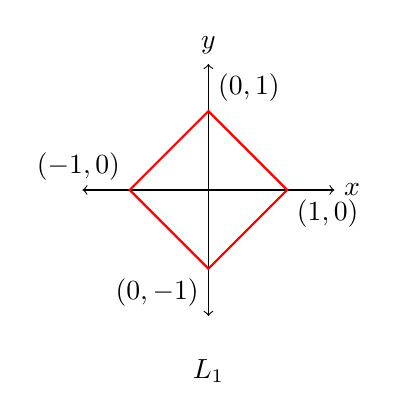
\begin{tikzpicture}
    \draw[very thin,gray] (-2,-2) (2,2);
    \draw[<->] (-1.6,0) node[left]{}--(1.6,0) node[right]{$x$};
    \draw[<->] (0,-1.6) node[left]{}--(0,1.6) node[above]{$y$};
    \draw[thick,red] (1,0) -- (0,1) --(-1,0) --(0,-1)--cycle;
    \draw(1,0) node[below right]{$(1,0)$};
    \draw(0,1) node[above right]{$(0,1)$};
    \draw(-1,0) node[above left]{$(-1,0)$};
    \draw(0,-1) node[below left]{$(0,-1)$};
    \node at (0,-2.3) {$L_{1}$};
\end{tikzpicture}
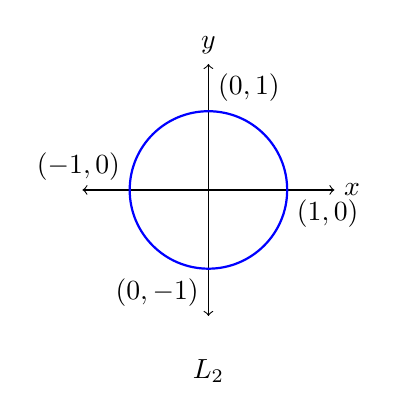
\begin{tikzpicture}
    \draw[very thin,gray] (-2,-2) (2,2);
    \draw[<->] (-1.6,0) node[left]{}--(1.6,0) node[right]{$x$};
    \draw[<->] (0,-1.6) node[left]{}--(0,1.6) node[above]{$y$};
    \draw[thick,blue] (0,0)circle[radius=1];
    \draw(1,0) node[below right]{$(1,0)$};
    \draw(0,1) node[above right]{$(0,1)$};
    \draw(-1,0) node[above left]{$(-1,0)$};
    \draw(0,-1) node[below left]{$(0,-1)$};
    \node at (0,-2.3) {$L_{2}$};
\end{tikzpicture}
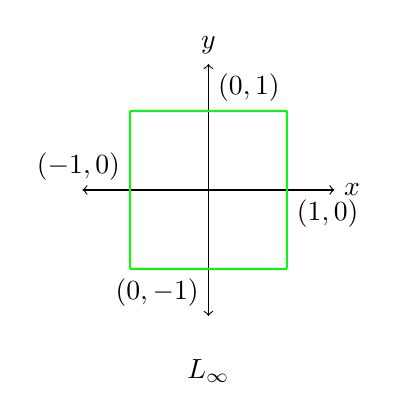
\begin{tikzpicture}
    \draw[very thin,gray] (-2,-2) (2,2);
    \draw[<->] (-1.6,0) node[left]{}--(1.6,0) node[right]{$x$};
    \draw[<->] (0,-1.6) node[left]{}--(0,1.6) node[above]{$y$};
    \draw[thick,green] (-1,1) rectangle (1,1);
    \draw[thick,green] (1,1) rectangle (1,-1);
    \draw[thick,green] (1,-1) rectangle (-1,-1);
    \draw[thick,green] (-1,-1) rectangle (-1,1);
    \draw(1,0) node[below right]{$(1,0)$};
    \draw(0,1) node[above right]{$(0,1)$};
    \draw(-1,0) node[above left]{$(-1,0)$};
    \draw(0,-1) node[below left]{$(0,-1)$};
    \node at (0,-2.3) {$L_{\infty}$};
\end{tikzpicture}
\]
\[
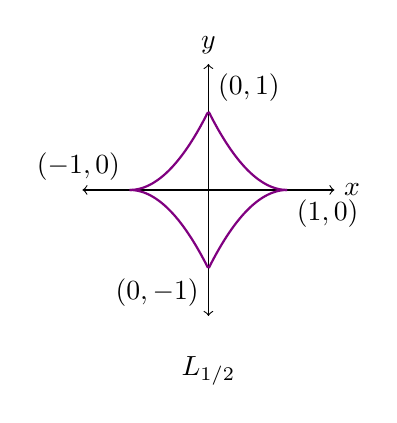
\begin{tikzpicture}
    \draw[very thin,gray] (-2,-2) (2,2);
    \draw[<->] (-1.6,0) node[left]{}--(1.6,0) node[right]{$x$};
    \draw[<->] (0,-1.6) node[left]{}--(0,1.6) node[above]{$y$};
    \draw[thick,violet,domain=-1:1,samples=100,smooth,variable=\x] plot({\x},{pow(1-abs(\x),2)});
    \draw[thick,violet,domain=-1:1,samples=100,smooth,variable=\x] plot({\x},{-pow(1-abs(\x),2)});
    \draw(1,0) node[below right]{$(1,0)$};
    \draw(0,1) node[above right]{$(0,1)$};
    \draw(-1,0) node[above left]{$(-1,0)$};
    \draw(0,-1) node[below left]{$(0,-1)$};
    \node at (0,-2.3) {$L_{1/2}$};
\end{tikzpicture}
\begin{tikzpicture}
    \draw[very thin,gray] (-2,-2) (2,2);
    \draw[<->] (-1.6,0) node[left]{}--(1.6,0) node[right]{$x$};
    \draw[<->] (0,-1.6) node[left]{}--(0,1.6) node[above]{$y$};
    \draw[thick,orange] (0,0) -- (0,1);
    \draw[thick,orange] (0,0) -- (0,1);
    \draw[thick,orange] (0,0) -- (0,1);
    \draw[thick,orange] (0,0) -- (0,1);

    \draw[thick,orange] (0,0) -- (0,-1);
    \draw[thick,orange] (0,0) -- (0,-1);
    \draw[thick,orange] (0,0) -- (0,-1);
    \draw[thick,orange] (0,0) -- (0,-1);

    \draw[thick,orange] (0,0) -- (1,0);
    \draw[thick,orange] (0,0) -- (1,0);
    \draw[thick,orange] (0,0) -- (1,0);
    \draw[thick,orange] (0,0) -- (1,0);

    \draw[thick,orange] (0,0) -- (-1,0);
    \draw[thick,orange] (0,0) -- (-1,0);
    \draw[thick,orange] (0,0) -- (-1,0);
    \draw[thick,orange] (0,0) -- (-1,0);

    \draw(1,0) node[below right]{$(1,0)$};
    \draw(0,1) node[above right]{$(0,1)$};
    \draw(-1,0) node[above left]{$(-1,0)$};
    \draw(0,-1) node[below left]{$(0,-1)$};
    \node at (0,-2.3) {$L_{0}$};
\end{tikzpicture}
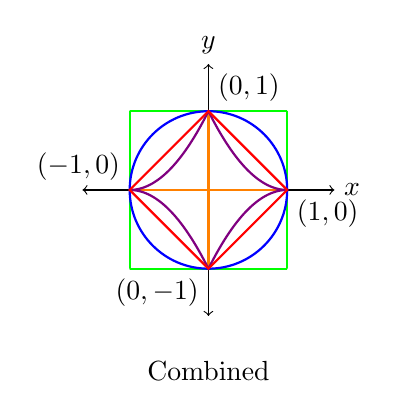
\begin{tikzpicture}
    \draw[very thin,gray] (-2,-2) (2,2);
    \draw[<->] (-1.6,0) node[left]{}--(1.6,0) node[right]{$x$};
    \draw[<->] (0,-1.6) node[left]{}--(0,1.6) node[above]{$y$};
    \draw[thick,orange] (0,0) -- (0,1);
    \draw[thick,orange] (0,0) -- (0,1);
    \draw[thick,orange] (0,0) -- (0,1);
    \draw[thick,orange] (0,0) -- (0,1);

    \draw[thick,orange] (0,0) -- (0,-1);
    \draw[thick,orange] (0,0) -- (0,-1);
    \draw[thick,orange] (0,0) -- (0,-1);
    \draw[thick,orange] (0,0) -- (0,-1);

    \draw[thick,orange] (0,0) -- (1,0);
    \draw[thick,orange] (0,0) -- (1,0);
    \draw[thick,orange] (0,0) -- (1,0);
    \draw[thick,orange] (0,0) -- (1,0);

    \draw[thick,orange] (0,0) -- (-1,0);
    \draw[thick,orange] (0,0) -- (-1,0);
    \draw[thick,orange] (0,0) -- (-1,0);
    \draw[thick,orange] (0,0) -- (-1,0);
    \draw[very thin,gray] (-2,-2) (2,2);
    \draw[thick,violet,domain=-1:1,samples=100,smooth,variable=\x] plot({\x},{pow(1-abs(\x),2)});
    \draw[thick,violet,domain=-1:1,samples=100,smooth,variable=\x] plot({\x},{-pow(1-abs(\x),2)});
    \draw[very thin,gray] (-2,-2) (2,2);
    \draw[thick,green] (-1,1) rectangle (1,1);
    \draw[thick,green] (1,1) rectangle (1,-1);
    \draw[thick,green] (1,-1) rectangle (-1,-1);
    \draw[thick,green] (-1,-1) rectangle (-1,1);
    \draw[very thin,gray] (-2,-2) (2,2);
    \draw[thick,blue] (0,0)circle[radius=1];
    \draw[very thin,gray] (-2,-2) (2,2);
    \draw[thick,red] (1,0) -- (0,1) --(-1,0) --(0,-1)--cycle;

    \draw(1,0) node[below right]{$(1,0)$};
    \draw(0,1) node[above right]{$(0,1)$};
    \draw(-1,0) node[above left]{$(-1,0)$};
    \draw(0,-1) node[below left]{$(0,-1)$};
    \node at (0,-2.3) {Combined};
\end{tikzpicture}
\]
\item \textbf{S-Norm} if $S$ is a symmetric matrix then $S-$Norm of a vector $v$ is defined as following

\begin{equation}
    \Vert v\Vert_S=\sqrt{\left(v^TSv\right)} \tag{S-Norm}
\end{equation}

\item \textbf{Minising the Norm on Curve} 

suppose we have a curve $C$ and we want to find the point on the tcurve that has minimum $L_p$ norm there are two ways 
\begin{itemize}
    \item Algebrically 
    \item Geometrically
\end{itemize}
example suppose curve $ax+by=1$ and we want to find the points on this line which has minimum $L_1,L_2$ norm

\textbf{1.Geometrically}
\[
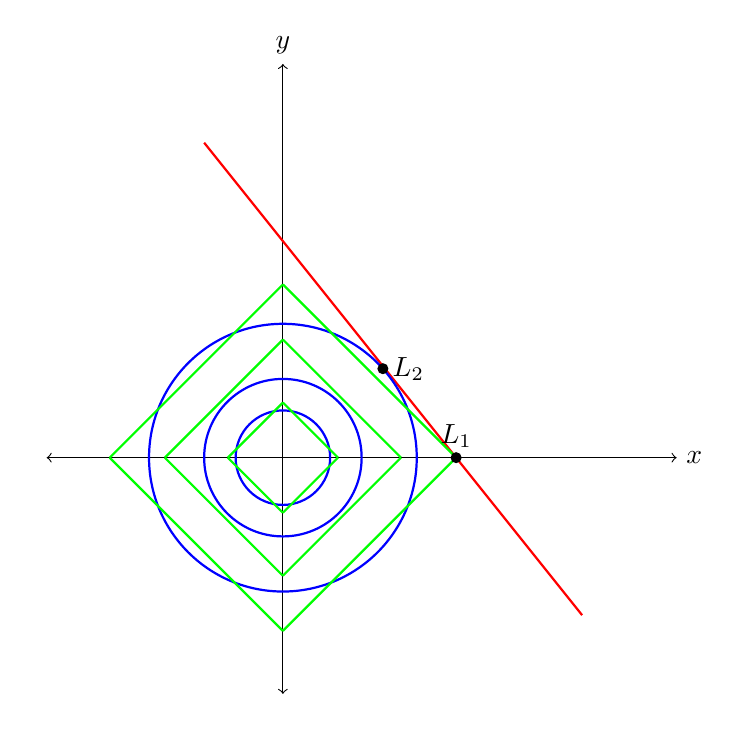
\begin{tikzpicture}
    \draw[very thin,gray] (-2,-2) (2,2);
    \draw[<->] (-3,0) node[left]{}--(5,0) node[right]{$x$};
    \draw[<->] (0,-3) node[left]{}--(0,5) node[above]{$y$};
    \draw[thick,red] (-1,4) -- (3.8,-2);
    \draw[thick,blue] (0,0) circle[radius=1.7];
    \draw[thick,blue] (0,0) circle[radius=0.6];
    \draw[thick,blue] (0,0) circle[radius=1];
    \draw[thick,green] (0,0.7)--(-0.7,0);
    \draw[thick,green] (0.7,0)--(0,-0.7);
    \draw[thick,green] (-0.7,0)--(0,-0.7);
    \draw[thick,green] (0.7,0)--(0,0.7);
    \draw[thick,green] (0,1.5)--(-1.5,0);
    \draw[thick,green] (1.5,0)--(0,-1.5);
    \draw[thick,green] (-1.5,0)--(0,-1.5);
    \draw[thick,green] (1.5,0)--(0,1.5);
    \draw[thick,green] (0,2.2)--(-2.2,0);
    \draw[thick,green] (2.2,0)--(0,-2.2);
    \draw[thick,green] (-2.2,0)--(0,-2.2);
    \draw[thick,green] (2.2,0)--(0,2.2);
    \fill[black](2.2,0)circle(2pt);
    \fill[black](1.27,1.13)circle(2pt);
    \node[above] at (2.2,0) {$L_{1}$};
    \node[right] at (1.27,1.13) {$L_{2}$};
\end{tikzpicture}
\]
we know the picture of $L_1,L_2$ norm so for a particular norm starting from normvalue=0 we expand the picture the first intersection with the figure gives the point where that norm is minimum.

for $L_2$ norm we expanded the circle and for $L_1$ we expand diamond.

\textbf{2.Algebrically}

$L_1$ norm will minimum at the closest sparsest point or where the maximum number of components are 0.

$L_2$ we will write the general equation of circle with center at original and radius r, $x^2+y^2=r^2$ then solve with the curve for tangent.
\item \textbf{Norm of Matrices} Here are few types of matrix norms for matrix $A_{m\times n}$

\textbf{$\circledast$ $\mathbf{\Vert A \Vert_2}\rightarrow$} it is equal to maximum singular value in SVD form of the matrix.
\[\Vert A \Vert_2=max\left(\frac{\Vert A\vec{v} \Vert}{\Vert \vec{v} \Vert}\right)\]
as we know that $A\vec{v}_i=\sigma_i \vec{v}_i$ so it will be maximum for $\sigma_1,\vec{v}_1$ 
\[\therefore \Vert A \Vert_2=max\left(\frac{\Vert A\vec{v} \Vert}{\Vert \vec{v} \Vert}\right)=\sigma_1\]

\textbf{$\circledast$ $\mathbf{\Vert A \Vert_F}\rightarrow$} it is defined as Sqrt of sum of squares of all elements in the matrix, also known as \textbf{Frobenius Norm}.
\[\Vert A \Vert_F=\left(\sum_{i=1}^{m}\sum_{j=1}^{n}A_{ij}\right)^{1/2}\]

note as $A=u\Sigma v^T$ and $u,v$ are orthogonal matrices therefore
\[\Vert A \Vert_F=\Vert \Sigma \Vert_F=\left(\sum_{}^{}(\sigma_i)^2\right)^{1/2}\]
\textbf{$\circledast$ $\mathbf{\Vert A \Vert_N}\rightarrow$} it is defined as sum of singular values($\sigma_i$) this norm is also known as \textbf{Nuclear Norm}.
\[\Vert A \Vert_N=\sum_{}^{}\sigma_i\]
\textbf{Note: }$\Vert A \Vert_2,\Vert A \Vert_F,\Vert A \Vert_N$ only depends on singular values $\sigma_1,\sigma_2\dots,\sigma_n$\\
\textbf{Note: }Zero Norm of a matrix is defined as rank of matrix.

\item \textbf{Principle Component Analysis(PCA)}

if we have a matrix $A$ rank $r$ and we have arbitrary another matrix $B$ of rank $k\leq r$, then according to \textbf{Eckart Young Theorem}

\[\boxed{\Vert A-B\Vert \geq \Vert A-A_k \Vert}\]
where $A_k$ is diagonal matrix with largest $k$ singular values of its $\sigma_i$'s 

example let we have a matrix $A$ of order $4\times 4$
\[\begin{bmatrix}
    4&0&0&0\\
    0&3&0&0\\
    0&0&2&0\\
    0&0&0&1\\
\end{bmatrix}\]

then for all matrices $B$ of rank $k\leq 4$ $\rightarrow$ $\Vert A-B\Vert_k \geq \Vert A-A_k\Vert$ taking $k=2,$ $\Vert A-B\Vert \geq \Vert A-A_2\Vert$ here $A_2$ will be 
\[\begin{bmatrix}
    4&0&0&0\\
    0&3&0&0\\
    0&0&0&0\\
    0&0&0&0\\
\end{bmatrix}\]
\\
\begin{center}
    \textbf{\Huge{Lecture-8}}
\end{center}
\item \textbf{Ways to Solve Least Square Problems($A_{m\times n}$)}

\textbf{1.$\mathbf{A^TA{x}=A^T{b}}(m>n)$}

Basically we are trying to minimize the error, $\vec{e}=A\vec{x}-\vec{b}$ we will minimize its $L_2$ norm which is $\Vert \vec{e} \Vert^2$
\[\Vert \vec{e} \Vert^2=\Vert A\vec{x}-\vec{b} \Vert^2=(A\vec{x}-\vec{b})^T(A\vec{x}-\vec{b})\]
\[\Vert \vec{e} \Vert^2=\vec{x}^TA^TA\vec{x}-\vec{x}^TA^T\vec{b}-\vec{b}^TA\vec{x}+\vec{b}^T\vec{b}\]
after solving it for minimum we will get $\vec{x}=(A^TA)^{-1}A^T\vec{b}$

Assumption: $A$ has full column rank because then only $A^TA$ is invertible
\\

\textbf{2.Pseudo Inverse}($\forall \hspace{3pt}m,n$)

if a matrix is invertible then everything is fine but for non-invertible matrices we define the concept of Pseudo Inverse, which is closest to inverse as much as possible if $A_{m\times n}=u\Sigma v^T$ rank $r$ then
\begin{equation}
    A^{+}=v\Sigma^+u^T \tag{Pseudo Inverse}
\end{equation}
where $\Sigma^+$ is pseudo inverse of $\Sigma$ as much as possible!

$\circledast$ How to solve $A\vec{x}=\vec{b}$ using pseudo inverse?

$\circledast$ When there is no inverse, our claim is that $\vec{x}=A^+\vec{b}$ fits the best in the equation $A\vec{x}=\vec{b}$ or $\Vert A\vec{x}-\vec{b}\Vert_2$  is minimum for $\vec{x}=A^+\vec{b}$ as $A^+=(A^TA)^{-1}A^T$ can be proved.
\\

\textbf{3.Undetermined$(m<n)$} 

we can use $\vec{x_1}=A^+\vec{b}$ which is a minimizing $L_2$ norm but we can find $\vec{x_2} $ by minimizing $L_1$  norm. this case is quite useful in Deep Learning
\\

\textbf{4.$\mathbf{\Vert Ax-b\Vert^2+{{\delta}^2\Vert x\Vert^2}}$} when $A$ is near singular this method can be used.

Note:Here ellimination will not give satisfying results on solving for x
\\

suppose we minimize $\Vert Ax-b\Vert^2+{{\delta}^2\Vert x\Vert^2}$ then we can write 
\[\begin{bmatrix}
    A\\\delta I
\end{bmatrix}\begin{bmatrix}
    \vec{x}
\end{bmatrix}=\begin{bmatrix}
    \vec{b}\\\vec{0}
\end{bmatrix}
\]
say $\begin{bmatrix}
    A\\\delta I
\end{bmatrix}=A^*$ and $\begin{bmatrix}
    \vec{b}\\\vec{0}
\end{bmatrix}=\vec{b}^*$, so $A^*\vec{x}=\vec{b}^*$ and hence the solution will be
\[(A^*)^TA^*\vec{x}=(A^*)^T\vec{b}^* \hspace{4pt} \rightarrow \hspace{4pt} A^TA+\delta^2 I\vec{x}=A^T\vec{b}\]

\textbf{Que:} But what is $\delta$ and how to find it?\\
\textbf{Ans:} $Later!$ for now let us see what will happen if $\delta \rightarrow 0$

suppose $A$ is $1\times 1$ matrix $A=\begin{bmatrix}\sigma \end{bmatrix}$, so our solution become $\sigma^2+\delta^2 \vec{x}=\sigma \vec{b}$
\[\vec{x}=\frac{\sigma \vec{b}}{\sigma^2+\delta^2 }\]

here we are just minimizing $(\sigma \vec{x}-\vec{b})^2+\delta^2x^2$ which we can do using calculus as well gives the same result $Analysising \hspace{4pt}as \hspace{4pt} \delta\rightarrow0$
\[\vec{x} \rightarrow 
\begin{cases}
    \vec{b}/{\sigma} \hspace{0.5cm} \sigma>0\\
    0 \hspace{0.85cm} \sigma=0\\
\end{cases}\]
$Conclusion \rightarrow$ as $\delta \rightarrow0$ $\vec{x} \rightarrow A^+\vec{b}$ where $A^+$ is pseudo inverse.

it was not a proof but can be done using SVD form \& the big result is that w.r.t $L_2$ norm the solution is\[\vec{x}=A^+\vec{b}=(A^TA+\delta^2I)^{-1}A^T \vec{b}\]

\textbf{Que: }What if we minimize $A\vec{x}-\vec{b}$ w.r.t $L_2$ and $\delta^2\vec{x}$ w.r.t $L_1$ norm?
\[minimize((\Vert A\vec{x}-\vec{b}\Vert_2)^2+\delta^2(\Vert \vec{x}\Vert_1)^2)\]

its know as $Lasso$!
\\

\textbf{5.Gram Schimit} when columns are in \textbf{*}bad condition then first of all we will orthogonolize $A$ ($A=QR$). it can we done in two ways
\textbf{*}bad condition means it is possible that columns are nearly dependent!
\begin{itemize}
    \item Usual Projection way$\rightarrow$ as new vector comes in keep elliminating projections on already calculated orthogonal vectors($ref-$18.06).
    \item Column Pivoting$\rightarrow$ it involves the swapping of columns (if required).if we have $a_1,a_2\dots,a_n$ as our columns of the matrix then 
    \begin{itemize}
        \item choose biggest $L_2$ normed out of $a_1,a_2\dots,a_n$.
        \item next vector($a_i$) out of remaining columns we will choose such that $\Vert a_i\Vert_2-P(a_i)$ is maximum.
        where $P(a_i)$ is the projection of $a_i$ on already found orthogonal vector.
    \end{itemize}
\end{itemize}

\textbf{6.Krylov} when $A$ is large sparse matrix

first we calculate krylov's space $K_j$ then we use those basis to solve $A\vec{x}=\vec{b}$
\[K_j=\{\vec{b},A\vec{b},A^2\vec{b}\dots,A^{j-1}\vec{b}\}\]
we can improve this method by orthogonolizing basis of $K_j$ it is done by method which was figured out by \textbf{Arnoldi \& Lanczos}

\textbf{Books} recomendations for numerical Linear Algebra
\begin{itemize}
    \item Trefethen-because
    \item Golub and Vanloan
\end{itemize}


\begin{center}
    \textbf{\Huge{Lecture-9}}
\end{center}

\item \textbf{Computing EigenValues}

One of the method to compute eigenvalues is by setting $A-\lambda I$ to 0 then compute for eigenvalues but w.k.t as order of matrix increases($\geq 5$) its very hard to find the eigenvalues.

to find the $Approx$ eigenvalues we use following method even $matlab$ and other maths software uses this method. here are the steps


\textbf{1.} Write, $A=A_0=Q_0R_0$ , $Q_0$ is orthogonal \& $R_0$ is upper triangular\\
\textbf{2.} Use, $A_n=R_nQ_n$ $\forall$ $n \in \{1,2\dots,n\}$
\begin{itemize}
    \item $A_0,A_1\dots,A_n$ will have same eigenvalues as they are similar!
    \item $Accuracy \propto n$
\end{itemize}

More Improvement can be done in this method using Shifts before the step 1 and after the step 2

\textbf{0.} Subtract $sI$ form $A$ or $A_0$\\
\textbf{4.} Add $sI$ to $A_n$

even more can be improved by reducing the matrix to $hessenberg$ $form$ first then start with the step 0.

\textbf{Note:} if the matrix is symmetric then it will stay symmetric in the whole process and its hessenberg form will be a tridiagonal matrix.

\item \textbf{Hessenberg Matrix}

when matrix is almost upper triangular except the diagonal near the main diagonal is non-zero


\[\begin{bmatrix}
    * &*&\dots&*&*\\
    *&*&\dots&*&*\\
    \vdots&\vdots&*&*&\vdots\\
    0&0&*&\ddots&*\\
    0&0&\dots&*&*

\end{bmatrix}\]

\item \textbf{Computing Singular Values}

w.k.t singular values are the square root of eigenvalues of $A^TA$ so one way is to compute $A^TA$ then calculate its eigenvalues but calculating $A^TA$ for huge matrices will be a time consuming step (by computers) therefore another method is \dots

\textbf{1.} Write $A=u\Sigma v^T$ \\
\textbf{2.} Multiply by orthogonal matrices $Q_1$ and $Q_2$ s.t $A$ becomes bidiagonal martrix $(Q_1u\Sigma v^T Q_2)$, as multiplying by orthogonal matrices does not affect the singular values.\\
\textbf{3.} hence $A^TA$ will be tridiagonal
\textbf{4.} Use Eigenvalues method.\\
\\
\begin{center}
    \textbf{\Huge{Lecture-10}}
\end{center}

\item \textbf{Randomized Matrix Multiplication}

suppose we have two matrix $A$ with columns $a_1,a_2\dots,a_k$ and $B$ with rows $b_1,b_2\dots,b_k$ then w.k.t usual multiplication of $A,B$ is 
\[A=\begin{bmatrix}
    \uparrow &\uparrow &\dots&\uparrow\\
    a_1&a_2&\dots&a_k\\
    \downarrow &\downarrow &\dots&\downarrow\\
\end{bmatrix} \hspace{4pt}and \hspace{4pt} B=\begin{bmatrix}
    \leftarrow&b_1&\rightarrow\\
    \leftarrow&b_2&\rightarrow\\
    \vdots&\vdots&\vdots\\
    \leftarrow&b_k&\rightarrow\\
\end{bmatrix}\]
\[M=A\times B=\sum_{i=0}^{k}a_ib_i\]

but in randomized matrix multiplication we consider product of columns of $A$ \& rows of $B$ as sample space as follows 
\[Sample \hspace{4pt} Space \hspace{4pt} S=\{s_i=a_ib_i\hspace{4pt} | \hspace{4pt} i\in \{1,2\dots,k\}\}\]

with the probabilities $p_i$.
\[\sum_{i=1}^{k}p_i=1\]

Prerequisites$\longrightarrow$ Mean($\mu$),Varience($\sigma^2$),Standard Deviation($\sigma$)\dots
\[\mu =\sum p_i*s_i\]
\[\sigma^2=\sum p_i*(s_i-\mu)^2=\left(\sum p_is_i^2\right)-()\mu^2)\]

\[ \sigma=\sqrt{varience}\]

\textbf{Note: }In randomized matrix multiplication Mean($\mu$) of all the samples will always be correct we'll focus on to minimize the Varience($\sigma^2$) by choosing appropriate probability distribution.\\

\textbf{Que} But what should be the $Probability$ $Distribution$?\\
\textbf{Ans} $Norm$ $Squared$ $Distribution!$ turns out to be the best

\begin{equation}
    p_i=\frac{\Vert a_i \Vert \times \Vert b_i \Vert}{C} \hspace{4pt} , \hspace{4pt} C=\sum_{j=1}^{k}\Vert a_j \Vert  \times \Vert b_j \Vert
\end{equation}

hence approx multiplication $AB$ for $1$ sample out of $n$ will be
\[approx(AB)=\sum_{i=1}^{k}p_i \times \left(\frac{a_ib_i}{np_i}\right)=\sum_{i=1}^{k}\frac{1}{n}\left(a_ib_i\right)\]
therefore Mean($\mu$) of whole sample space would be
\[\mu=\sum_{i=1}^{k}a_ib_i=AB\]
which is correct as it matches with original multiplication.

now calculating varience of the for 1 sample
\[=\left(\sum_{i=1}^{k}\frac{p_i}{n}\left(\frac{\Vert a_i\Vert \Vert b_i\Vert}{p_i}\right)^2\right)-\frac{1}{n}\left(\Vert AB\Vert_F\right)^2\]
\[=\left(\sum_{i=1}^{k}\frac{1}{np_i}\left({\Vert a_i\Vert \Vert b_i\Vert}\right)^2\right)-\frac{1}{n}\left(\Vert AB\Vert_F\right)^2\]

substituting value of $p_i$ from eq(0.1) we will get
\[=\frac{C}{n}\left(\sum_{i=1}^{k}\left({\Vert a_i\Vert \Vert b_i\Vert}\right)\right)-\frac{1}{n}\left(\Vert AB\Vert_F\right)^2\]
\[=\frac{C^2}{n}-\frac{1}{n}\left(\Vert AB\Vert_F\right)^2=\frac{1}{n}\left(C^2-\left(\Vert AB\Vert_F\right)^2\right)\]




then for the whole sample varience($\sigma$) would be 
\[\sigma^2=C^2-\left(\Vert AB\Vert_F\right)^2\]
Clearly $\left(\Vert AB\Vert_F\right)^2$ is a constant term so we have to minimize $C$.

\textbf{Claim: }C is minimum for Norm Squared Distribution!\\
\textbf{Proof: }It uses \textbf{Lagrange Multiplier} method
\[Target \rightarrow minimize\left(f(p_i)=\frac{\Vert a_i\Vert^2 \Vert b_i\Vert^2}{p_i}\right)\]
\[Constraint \rightarrow \sum p_i=1\]
Lagrange Multiplier says that write net minimizing function as 
\[f(p_i,\lambda)=Target+\lambda(Constraint)\]
\[f(p_i,\lambda)=f(p_i)+\lambda\left(\sum p_i-1\right)\]
now use calculus and get the solution
\begin{equation}
    \frac{\partial\left(f(p_i,\lambda)\right)}{\partial p_i}=0 \implies -\frac{\Vert a_i\Vert^2 \Vert b_i\Vert^2}{p_i^2}+\lambda=0
\end{equation}
\begin{equation}
    \frac{\partial\left(f(p_i,\lambda)\right)}{\partial \lambda}=0 \implies \sum p_i=0
\end{equation}
from eq(0.2)
\[p_i=\sqrt{\frac{\Vert a_i\Vert^2 \Vert b_i\Vert^2}{\lambda}}=\frac{\Vert a_i\Vert \Vert b_i\Vert}{\sqrt{\lambda}} \hspace{4pt},\hspace{4pt}\sqrt{\lambda}=C\]

\begin{center}
    \textbf{\Huge{Lecture-11}}
\end{center}
\vspace{5pt}
\item \textbf{Low Rank Matrices}

what will be the inverse of an Identity matrix after rank-1 perturbation or what is the inverse of $I-uv^T$ where $I$ is order $n$ matrix and $u,v\in \mathbb{R}^n$\\

Claim:
\[ \boxed{(I-uv^T)^{-1}=I+\frac{uv^T}{1-v^Tu}}\]
Proof:
\[ \left(I-uv^T\right)\left(I+\frac{uv^T}{1-v^Tu}\right)\]
\[=I^2+\frac{uv^T}{1-v^Tu}-uv^T-\frac{uv^Tuv^T}{1-v^Tu}\]
\[=I+\frac{(I-uv^T)uv^T}{1-v^Tu}-uv^T\]
\[=I+\frac{(I-uv^T)uv^T-(I-uv^T)uv^T}{1-v^Tu}=I+0=I\]

what if we do $rank-k$ perturbation ?

suppose we have an Identity matrix of order $n\times n$ and matrix $U$ of order $n\times k$ with k independent columns also a matrix $V$ of order $ktimes n$ with k independent rows \\

Claim:
\[ \boxed{(I_n-UV^T)^{-1}=I_n+{U\left({(I_k-V^TU})^{-1}\right)V^T}}\]
Proof:
\[(I_n-UV^T)\left(I_n+{U\left({(I_k-V^TU})^{-1}\right)V^T}\right)\]
\[=(I_n-UV^T)I_n+(I_n-UV^T)\left({U\left({(I_k-V^TU})^{-1}\right)V^T}\right)\]
\[=I_n-UV^T+(I_n-UV^T)U\left({\left({(I_k-V^TU})^{-1}\right)V^T}\right)\]
\[=I_n-UV^T+U(I_k-V^TU)\left(I_k+V^TU\right)^{-1}V^T\]
\[I_n-UV^T+UI_kV^T=I_n\]

\textbf{Applications:}
\begin{itemize}
    \item to solve $(I-uv^T)\vec{x}=\vec{b}$
    \item new measurement in least squares(old was ($A\vec{x}=\vec{b}$)) and normal equation was $A^TA\vec{x}=A^T\vec{b}$ now new normal equation is \textbf{dynamic}
    \[\begin{bmatrix}
        A^T&v
    \end{bmatrix}\begin{bmatrix}
        A\\v^T
    \end{bmatrix}\hat{x}_{new}=\begin{bmatrix}
        A^T&v
    \end{bmatrix}\begin{bmatrix}
        \vec{b}\\b_{new}
    \end{bmatrix}\]
    \[(A^TA+vv^T)\hat{x}_{new}=A^Tb+v\vec{b}_{new}\]
\end{itemize}

\textbf{Note$^1$: }This formula was derived by $Sherman,Morison,Woodbury(SMW)$ but it is also know as \textbf{Matrix Inversion}.\\
\textbf{Note$^2$: } Kalman Filter uses this Idea of dynamic normal equations\\

now suppose we have a system of equation to solve $Aw=b$ for $w$ and then we want to solve $(A-uv^T)x=b$  for $x$ then do find the $x$ quickly using previous determined data we do the following.
\begin{itemize}
    \item Solve equation $Az=b$ for $z$
    \item \& we have solution to the equation $Aw=b$ for $w$
    \item Combine both to get $x$
    \[\boxed{x=w+\frac{wv^Tz}{1-v^Tz}}\]
\end{itemize}

\textbf{Generalization of SMW} 

for any square matrix $A_{n\times n}$ and $u,v$ be the $rank-k\leq n$ matrix with order $n\times k$ and $k\times n$ respectively
\[\boxed{(A-uvT)^{-1}=A^{-1}-A^{-1}u\left(I-v^TA^{-1}u\right)^{-1}v^TA^{-1}}\]

\textbf{Note:} $rank-k$ perturbation in matrix will perturb its inverse by $rank-k$\\
\begin{center}
    \textbf{\Huge{Lecture-12}}
\end{center}
\vspace{5pt}

\item \textbf{Time Dependent Matrices}

let us have a matrix $A(t)$ is function of time then how would $A^{-1}(t)$ changes as times varies?

\textbf{Que:} Mathematically we are given $\frac{dA(t)}{dt}$ and we have to find $\frac{dA^{-1}(t)}{dt}$\\

\textbf{Solution:} let initially we had matrix $A$ then it is changed to $B=A+\Delta A$ the using the following identity

\[\boxed{B^{-1}-A^{-1}=B^{-1}(A-B)A^{-1}}\]

\[(\Delta A)^{-1}=(A+\Delta A)^{-1}(-\Delta A)(A^{-1})\]
dividing by $\Delta t$,
\[\left(\frac{\Delta A^{-1}}{\Delta t}\right)=\left(A+\Delta A\right)^{-1}\left(\frac{-\Delta A}{\Delta t}\right)(A^{-1})\]
as $\Delta t\rightarrow 0$
\[\boxed{\frac{d A^{-1}}{d t}=-A^{-1}\left(\frac{d A}{d t}\right)(A^{-1})}\]

\item \textbf{Time Dependent Eigenvalues} 

Here are few facts(results) before starting
\begin{itemize}
    \item Standard Eigenvalue Defination $\rightarrow{{A(t){x}(t)=\lambda(t){x}(t)}} \hspace{7pt}---(1)$
    \item Transpose have same eigenvalues $\rightarrow{{y^T(t)A(t)=\lambda(t){y^T}(t)}} \hspace{7pt}---(2)$
    \item Normalization $\rightarrow{y^Tx=1}$ 
    \item $AX=XA$ \& $Y^TA=AY^T$ where $X$ \& $Y$ are eigenvector matrix
    \item from 1,2 $\rightarrow$ $y^T(t)A(t)x(t)=\lambda(t)$
\end{itemize}

\textbf{Note:} When $A$ will be symmetric $y^Ty=1$  represents unit vector.
\[\frac{d(\lambda(t))}{dt}=\frac{d\left(y^T(t)A(t)x(t)\right)}{dt}\]
\[\frac{d(\lambda(t))}{dt}=\frac{d(y^T(t))}{dt}A(t)x(t)+y^T(t)\frac{d(A(t))}{dt}x(t)+y^TA(t)\frac{d(x(t))}{dt}\]

using (1),(2) 
\[\frac{d(\lambda(t))}{dt}=\frac{d(y^T(t))}{dt}\lambda(t)x(t)+y^T(t)\frac{d(A(t))}{dt}x(t)+\lambda(t)y^T(t)\frac{d(x(t))}{dt}\]

\[\frac{d(\lambda(t))}{dt}=\lambda(t)\frac{d\left(y^T(t)x(t)\right)}{dt}+y^T(t)\frac{d(A(t))}{dt}x(t)\]
as $y^T(t)x(t)=1$

\[\boxed{\frac{d(\lambda(t))}{dt}=y^T(t)\frac{d(A(t))}{dt}x(t)}\]

$x(t)$ and $y^T(t)$ are know as right and left eigenvectors respectively at time $t$\\

\textbf{*Interlacing theorem:}  if $S_{n\times n}$ is a symmetric matrix with eigenvalues $\gamma_1\geq \gamma_2\dots\geq \gamma_n$ and $\vec{u}\in \mathbb{R}^n$ then eigenvalues of $S+uu^T$,  $\lambda_1\geq \lambda_2\dots\geq\lambda_n$ will be such that
\[\boxed{\lambda_1 \geq \gamma_1 \geq \lambda_2 \geq \gamma_2  \dots\geq \lambda_n \geq \gamma_n}\]
if we add more $rank-1$ terms to $S$ it will behave same way example let $w\in \mathbb{R}^n$ then eigenvalues of $S+uu^T+ww^T$, $\alpha_1\geq \alpha_2\dots\geq \alpha_n$ then
\[{{\alpha _1 \geq\lambda_1 } \geq {\alpha _2 \geq\lambda_2 }  \dots\geq {\alpha _n \geq\lambda_n }}\]
we can relate $\alpha's$ and $\gamma's$ using both inequlities and also this theorem can be prooved usign Weyl's Inequality($ref-$NextLecture)\\

\textbf{Note:} $uu^T$ will be $rank-1$ positive semi-definate and one of its eigenvalue is $u^Tu>0$ and other 0's also eigenvector corrosponding to $u^Tu$ is $u$.\\

\textbf{Que:} What will happen if $u$ is an eigenvector of $S$ itself or ($Su=\lambda_i u$)\\
\textbf{Ans:} it means eigenvalue of $S+\theta uu^T$ corrosponding to $u$ will be $\lambda_i+\theta$
\[(S+\theta uu^T)u=Su+\theta uu^Tu=(\lambda_i+\theta)u\]
clearly we can see that as $\theta$ increases $\lambda_i+\theta>\{\lambda_{i-1},\lambda_{i-2}\dots,{\lambda_1}\}$ after certain point? \textbf{No!} if $\theta$ will increase then we'll swap this($\lambda_i+\theta$) eigenvalue with on of appropriate $\lambda_x \in \{\lambda_{i-1},\lambda_{i-2}\dots,{\lambda_1}\}$ so that Interlace Inequlity Theorem holds true\\

\begin{center}
    \textbf{\Huge{Lecture-13}}
\end{center}
\item \textbf{Derivative of A$^2$}
\[\frac{dA^2}{dt}=\lim_{\Delta t\rightarrow 0}\frac{\Delta A^2}{\Delta t} = \lim_{\Delta t\rightarrow 0} \frac{(A+\Delta A)^2-A^2}{\Delta t}\]
\[\frac{dA^2}{dt}=\lim_{\Delta t\rightarrow 0}\frac{A.\Delta A +\Delta A. A}{\Delta t}\]

\[\boxed{\frac{dA^2}{dt}=A\frac{dA}{dt}+\frac{dA}{dt}A}\]

\item \textbf{Time Dependent Singular Values}

\textbf{*}What we know 
\begin{itemize}
    \item $\sigma(t)=u^TAv$ where $u,v$ are unit vectors and A is matrix
    \item $v^Tv=1$ and $u^Tu=1$ therefore 
    \[\frac{dv^T}{dt}v+v^T\frac{dv}{dt}=0 \hspace{7pt} \& \hspace{7pt}\frac{du^T}{dt}u+u^T\frac{du}{dt}=0\]
as for vectors $x^Ty=y^Tx$ in real space($\mathbb{R}^n$)
\begin{equation}
    \frac{dv^T}{dt}v=v^T\frac{dv}{dt}=0 \hspace{7pt} \& \hspace{7pt}\frac{du^T}{dt}u=u^T\frac{du}{dt}=0
\end{equation}
\end{itemize}
\textbf{*}Derivation
\[\frac{d\sigma}{dt}=\frac{du^T}{dt}Av+u^T\frac{dA}{dt}v+u^TA\frac{dv}{dt}\]
\[\frac{d\sigma}{dt}=\frac{du^T}{dt}\sigma u+u^T\frac{dA}{dt}v+\sigma v^T\frac{dv}{dt}\]
using equation (0.4)
\[\frac{d\sigma}{dt}=0+u^T\frac{dA}{dt}v+0\]

\[\boxed{\frac{d\sigma}{dt}=u^T\frac{dA}{dt}v}\]

\item \textbf{Weyl's Inequality} 

for any 2 real symmetric matrices of same order $S,T$
\[\boxed{\lambda_{i+j-1}(S+T)\leq \lambda_i{S}+\lambda_j{T}}\]

\begin{center}
    \textbf{\Huge Lecture-14*}
\end{center}
\begin{center}
    \textbf{Prof: Alex Townsend}
\end{center}

\item \textbf{Why Low Rank Matrices}

let we have $rank-k$ matrix $X$ with singular values, $\sigma_1\geq \sigma_2\dots,\geq \sigma_n$ then we know the following facts
\begin{itemize}
    \item $rank(X)=k$
    \item $\sigma_{i}=0$, $\forall$ $i>k$
    \item $X=u_1v_1^T+u_2v_2^T\dots+u_kv_k^T$ $---(i)$
    \item $dim(R(X))=dim(C(X))=k$
\end{itemize}

\item \textbf{Defination of Low rank Matrix}

if we can share the matrix $X_{m\times n}$  information more efficiently(space wise) then $mn$, using $(i)$ we can send 2 matrix of order $m\times k$ and $k\times n$ instead of $X$ we say $X_{m\times n}$ is low rank when 
\[mk+kn<mn\]
or \[\boxed{k<\frac{mn}{m+n}}\]
for square matrices
\[k<\left(\frac{n^2}{2n}=\frac{n}{2}\right)\]

in practical world we demand more i.e. ($k\ll n/2$) to be more fast\\

\textbf{Que: }How do low rank matrices look like?\\
\textbf{Ans: }As rank decreases matrix get more aligned!

\textbf{Example1.} Lower triangular matrix with all ones on lower half and diagonal elsewhere zeros then this matrix \& its inverse are below

\[X=\begin{bmatrix}
    1&&&&\\
    1&1&&&\\
    1&1&1&&\\
    \vdots&\vdots&&\ddots&\\
    1&1&\dots&1&1
\end{bmatrix} \hspace{7pt}\& \hspace{7pt} X^{-1}=
\begin{bmatrix}
    1&&&&\\
    -1&1&&&\\
    &-1&1&&\\
    &&\ddots&\ddots&\\
    &&&-1&1
\end{bmatrix}
\]
\[X^TX=
\begin{bmatrix}
    1&-1&&&\\
    -1&2&-1&&\\
    &-1&2&-1&\\
    &&\ddots&\ddots&\ddots\\
    &&&-1&2&-1\\
    &&&&-1&2
\end{bmatrix}  \hspace{7pt}\& \hspace{7pt} \sigma_i(X)=\left[2sin\left(\frac{\pi(2i-1) }{2(2n+1)}\right)\right]^{-1}
\]

Graph of Ratio of ($\sigma_i(X)$ to $\sigma_1(X)$) vs ($i$)

\[
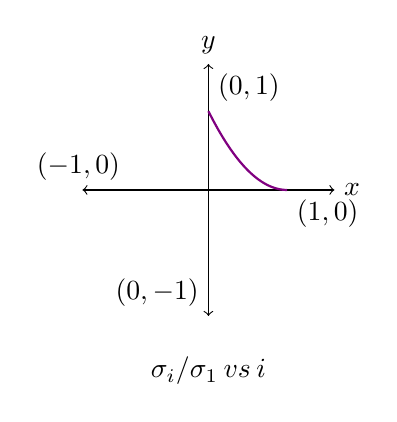
\begin{tikzpicture}
    \draw[very thin,gray] (-2,-2) (2,2);
    \draw[<->] (-1.6,0) node[left]{}--(1.6,0) node[right]{$x$};
    \draw[<->] (0,-1.6) node[left]{}--(0,1.6) node[above]{$y$};
    \draw[thick,violet,domain=0:1,samples=100,smooth,variable=\x] plot({\x},{pow(1-abs(\x),2)});
    \draw(1,0) node[below right]{$(1,0)$};
    \draw(0,1) node[above right]{$(0,1)$};
    \draw(-1,0) node[above left]{$(-1,0)$};
    \draw(0,-1) node[below left]{$(0,-1)$};
    \node at (0,-2.3) {$\sigma_i / \sigma_1 \hspace{2pt} vs \hspace{2pt} i$};
\end{tikzpicture}
\]
\textbf{Example2} Suppose we have following kind of matrix where non red area has 0 value
\[
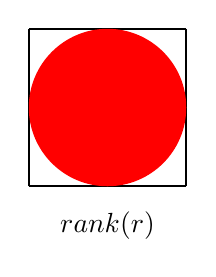
\begin{tikzpicture}
    \draw[thick,black] (-1,1)--(1,1);
    \draw[thick,black] (1,1)--(1,-1);
    \draw[thick,black] (1,-1)--(-1,-1);
    \draw[thick,black] (-1,-1)--(-1,1);
    \fill[red](0,0)circle(1cm);
    \node at (0,-1.5) {$rank(r)$};
\end{tikzpicture}\leq
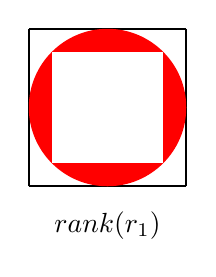
\begin{tikzpicture}
    \draw[thick,black] (-1,1)--(1,1);
    \draw[thick,black] (1,1)--(1,-1);
    \draw[thick,black] (1,-1)--(-1,-1);
    \draw[thick,black] (-1,-1)--(-1,1);
    \fill[red](0,0)circle(1cm);
    \fill[white](-0.707,-0.707)rectangle(0.707,0.707);
    \node at (0,-1.5) {$rank(r_1)$};
\end{tikzpicture}+
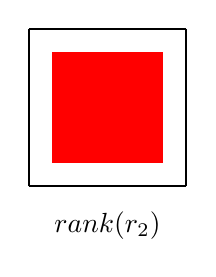
\begin{tikzpicture}
    \draw[thick,black] (-1,1)--(1,1);
    \draw[thick,black] (1,1)--(1,-1);
    \draw[thick,black] (1,-1)--(-1,-1);
    \draw[thick,black] (-1,-1)--(-1,1);
    \fill[red](-0.707,-0.707)rectangle(0.707,0.707);
    \node at (0,-1.5) {$rank(r_2)$};
\end{tikzpicture}
\]
but $rank(r_2)=1$, so $r\leq rank(r_1)+1$ and then we can use symmetry to break $r_1$ as well.\\

\item \textbf{Numerical Rank}

Numerical rank($rank_{\epsilon}$) of a matrix $X$ will be $k$, if for \underline{tolerence} $(0<\epsilon<1)$ 
\[\sigma_{k+1}(X) \leq \epsilon \sigma_1(X)\]
\[\sigma_{k}(X) > \epsilon \sigma_1(X)\]

assuming $\sigma_1\geq \sigma_2\dots\geq \sigma_n$

\textbf{Note: } $rank(X)=rank_{0}(X)$

\textbf{Eckart-Young: }$\sigma_{k+1}(X)=\Vert X-X_k \Vert_2$ How well X can be approximated!

\item \textbf{Numerical Low rank Matrices}
\begin{itemize}
    \item All low rank matrices
    \item Hilbert Matrices$\rightarrow$it is full rank matrix but very low numerical rank
    \[H_{ij}=\frac{1}{i+j-1}\]
    \item Vandermonde$\rightarrow$often we want $V^{-1}$ as $V$ is low numerical rank
    \[V=\begin{bmatrix}
        1&x_1&(x_1)^2&\dots&(x_1)^{n-1}\\
        1&x_2&(x_2)^2&\dots&(x_2)^{n-1}\\
        \vdots&\vdots&\vdots&&\vdots\\
        1&x_n&(x_n)^2&\dots&(x_n)^{n-1}\\
    \end{bmatrix}\]
\end{itemize}

\item \textbf{The World is Smooth$-$Reade(1893)}

if we take a polynomial and we form a matrix from integers sampling of this polynomial then that matrix will be 

\textbf{Example-} $P(x,y)=1+x+xy$ then matrix $X$ with entries $X_{ij}=P(i,j)$ happens to be numerically low rank! 
\[X=
\begin{bmatrix}
    1&1&\dots&1\\
    1&1&\dots&1\\
    \vdots&\vdots&\ddots&\vdots\\
    1&1&\dots&1\\
\end{bmatrix}+
\begin{bmatrix}
    1&1&\dots&1\\
    2&2&\dots&2\\
    \vdots&\vdots&\ddots&\vdots\\
    n&n&\dots&n\\
\end{bmatrix}+
\begin{bmatrix}
    1&2&\dots&n\\
    2&4&\dots&1\\
    \vdots&\vdots&\ddots&\vdots\\
    n&2n&\dots&n^2\\
\end{bmatrix}
\]
\[rank(X)\leq (1+1+1=3)\ll n\]

in general polynomial can be
\[P(x,y)=\sum_{i=0}^{m}\sum_{j=0}^{n}C_{ij}\left(x^iy^j\right) \hspace{4pt},\hspace{4pt} m<n\]
then rank of matrix $X$ with $X_{ab}=P(a,b)$ will be less than equal to $m^2$.

\item \textbf{The World is Sylvester} 

Matrices(X) satisfying the form $AX-XB=C$ for some $A,B,C$ then X is a numerical low rank
\[\sigma_{k+1}\leq Z_k(E,F)\sigma_1(X)\hspace{3.5pt},\hspace{3.5pt} rank(C)=r\]
$E,F$ are eigenvector matrices of $A,B$ respectively\\

\textbf{Example-}Hilbert Matrix,Vandermonde

\[
\begin{bmatrix}
    \frac{1}{2}&&&\\
    &\frac{3}{2}&&\\
    &&\ddots&\\
    &&&\frac{2n-1}{2}
\end{bmatrix}H-
H\begin{bmatrix}
    \frac{-1}{2}&&&\\
    &\frac{-3}{2}&&\\
    &&\ddots&\\
    &&&\frac{1-2n}{2}
\end{bmatrix}=
\begin{bmatrix}
    1&1&\dots&1\\
    1&1&\dots&1\\
    \vdots&\vdots&\ddots&\vdots\\
    1&1&\dots&1\\
\end{bmatrix}
\]
\[
\begin{bmatrix}
    x_1&&&\\
    &x_2&&\\
    &&\ddots&\\
    &&&x_n
\end{bmatrix}V-
V\begin{bmatrix}
    0&&&&-1\\
    1&0&&&\\
    &1&0&&\\
    &&\ddots&\ddots&\\
    &&&1&0
\end{bmatrix}=
\begin{bmatrix}
    0&0&\dots&0\\
    0&0&\dots&0\\
    \vdots&\vdots&\ddots&\vdots\\
    0&0&\dots&0\\
\end{bmatrix}
\]
\begin{center}
    \textbf{\Huge{Lecture-15}}
\end{center}
\item \textbf{Free Parameters}

Number of parameters required to know matrix are called free parameters
\begin{itemize}
    \item Square Matrix: $A_{n\times n}\rightarrow$ $n^2$
    \item Lower/Upper Triangular: $B_{n\times n}\rightarrow$ $n(n+1)/2$
    \item Lower/Upper Triangular with diagonal(1's): $C_{n\times n}\rightarrow$ $n(n-1)/2$
    \item Orthogonal Matrix: $Q_{n\times n}\rightarrow$ $n(n-1)/2$
    \item Diagonal Matrix: $\varLambda_{n\times n}\rightarrow$ $n$
    \item Symmetric Matrix: $S_{n\times n} \rightarrow$ $n(n+1)/2$
    \item Eigenvector Matrix: $E_{n\times n} \rightarrow$ $n^2-n$
\end{itemize}

different factorisation and there free parameters analysis

\begin{itemize}
    \item $A_{n\times n}=LU$ 
    \[\left(\frac{n(n-1)}{2}\right)+\left(\frac{n(n+1)}{2}\right)=n^2 \hspace{4pt} \checkmark \] 
    \item $A_{n\times n}=QR$ 
    \[\left(\frac{n(n-1)}{2}\right)+\left(\frac{n(n+1)}{2}\right)=n^2 \hspace{4pt} \checkmark\]
    \item $A_{n\times n}=X\varLambda X^{-1}$ 
    \[(n^2-n)+(n)+(0)=n^2  \hspace{4pt} \checkmark\]
    \item $A_{n\times n}=Q\varLambda Q^T$
    \[(n^2-n)+(n)+(0)=n^2  \hspace{4pt} \checkmark\]
    \item $A_{n\times n}=QS$
    \[\left(\frac{n(n-1)}{2}\right)+\left(\frac{n(n+1)}{2}\right)=n^2 \hspace{4pt} \checkmark\]
    \item SVD $A_{m\times n}=u\Sigma v^T$  Full rank matrix ($m\leq n$)
    \[\left(\frac{m(m-1)}{2}\right)+(m)+\left(mn-\frac{m(m+1)}{2}\right)=mn  \hspace{4pt} \checkmark\]
    \item SVD $A_{m\times n}=u\Sigma v^T$,  $rank-r<min(m,n)$
    \[\left(mr-\frac{r(r+1)}{2}\right)+(r)+\left(nr-\frac{r(r+1)}{2}\right)=mr+nr-r^2  \hspace{4pt} \checkmark\]
\end{itemize}

\item \textbf{Saddle Points} 

For a function or curve $f(x_1,x_2\dots,x_n)$ point $a=(a_1,a_2\dots,a_n)\in \mathbb{R}^n$ will be a saddle point if directional derivative of in all directions is 0 \& it is neither a maxima non a minima.

\textbf{Que: }From where saddle points arise?\\
\textbf{Ans: }There are 2 source of saddle points!\\

\textbf{1.} Suppose we have a symmetric matrix $S_{n\times n}$ and we want to minimize function $f(x)$ on the given $m$ constraints $A_{m\times n}(x)=b$ where $f(x)$ is
\[f(x)=\frac{1}{2}x^TSx ,\hspace{4pt} x\in \mathbb{R}^n \]

now if we have a Lagrangian $L(x,\lambda) =f(x)-\lambda^T(Ax-b)$\\

Claim: $L(x,\lambda)$ do not have max or min it has saddle point when $L'=0$\\

Proof: 
\[\frac{\partial L}{\partial x}=\frac{\partial }{\partial x}\left(\frac{1}{2}x^TSx-\lambda^T(Ax-b)\right)=Sx-A^T\lambda=0\]
\begin{equation}
    Sx=A^T\lambda
\end{equation}
\[\frac{\partial L}{\partial \lambda}=\frac{\partial }{\partial \lambda}\left(\frac{1}{2}x^TSx-\lambda^T(Ax-b)\right)=Ax-b=0\]
\begin{equation}
    Ax=b
\end{equation}
from equation (0.5),(0.6)
\[A'x'=b'\]
\begin{equation}
    \begin{bmatrix}
        S&A^T\\A&0
    \end{bmatrix} 
    \begin{bmatrix}
        x\\\lambda
    \end{bmatrix}=
    \begin{bmatrix}
        0\\b
    \end{bmatrix} \tag{KKT}
\end{equation}
doing ellimination on KKT matrix\\

\[
\begin{bmatrix}
    S&A^T\\A&0
\end{bmatrix}\xrightarrow[R_2-AS^{-1}R_1]{R_2=}
\begin{bmatrix}
    S&A^T\\0&-(AS^{-1}A^T)
\end{bmatrix}
\]
clearly KKT matrix ($A'$) has $n$ positive (as $n$ pivots of $S$ are positive) and $m$ negative eigenvalues(as $m$ pivots of $-AS^{-1}A^T$ are negative) therefore $x'$ is saddle point of $L$\\

\textbf{Note: }KKT$\rightarrow$ Karush,Kuhn,Tucker\\

\textbf{2.}Let $S$ is symmetric matrix , \textbf{Rayleigh Quotient} function is defined as
\[R(x)=\frac{x^TSx}{x^Tx}\]
\textbf{Note$^1$:} Max and Min values of $R(x)$ are $\lambda_1,\lambda_n$ for $x=q_1,q_n$ respectively. where $\lambda_1,\lambda_n$ are the max and min eigenvalues of $S$ and $q_1,q_n$ are corrosponding eigenvectors

\textbf{Note$^2$:} Here Saddle points are the Eigenvectors between $q_1$ \& $q_n$!

Example$\rightarrow$ suppose we have a diagonal matrix $D$ as follows
\[D=\begin{bmatrix}
    5&0&0\\
    0&3&0\\
    0&0&1\\
\end{bmatrix}\]

then rayleigh quotient function $R(x)$ will be
\[R(x)=\frac{x^TDx}{x^Tx}\]
let $x=(a,b,c)$ then 
\[R(x)=\frac{5a^2+3b^2+c^2}{a^2+b^2+c^2}\]
then $R(x)$ will have minima and maxima when $x$ is along the eigenvector corrosponding to $5,1$ respectively. and saddle point along the eigenvector corrosponding to $3$.

\textbf{Note: }Saddle point means maximum of a minimum of a function
\[\text{Saddle Point}\equiv max(min(f(x)))\]

\begin{center}
    \textbf{\Huge{Lecture-16}}
\end{center}

\item \textbf{Probability and Statistics Basic Terminologies}
\begin{itemize}
    \item Sample Mean($\bar{x}$) and Expected Mean($\mu$)
    \[\boxed{\bar{x}=\frac{1}{n}\sum_{i=1}^{n}x_i} \hspace{7pt} \boxed{\mu=\sum_{i=1}^{n}p_ix_i} \]
    \item Sample Varience($s^2$) and Expected Varience($\sigma^2$)
    \[ \boxed{s^2=\frac{1}{n-1}\sum_{i=1}^{n}(x_i-\bar{x})^2}\hspace{3pt}\boxed{\sigma^2=\sum_{i=1}^{n}p_i(x_i-\mu)^2=\left(\sum_{i=1}^{n}p_ix_i^2\right)-\mu^2}\]
    \item Expected value of $f(x)$
    \[E(f(x))=\sum_{i=1}^{n}p_if(x_i)\]
\end{itemize}
\textbf{Note: }for $f(x)=x$ and $f(x)=(x-\mu)^2$ expected value $\mathbb{E}(f(x))$ is expected mean and varience respectively.
\[\boxed{\mu=\mathbb{E}(x)} \hspace{5pt} \boxed{\sigma^2=\mathbb{E}((x-\mu)^2)=\mathbb{E}(x^2)-\mathbb{E}(x)^2}\]
\item \textbf{Markov's Inequality:} Probability of sample value greater than or equal to some number ($a$) is less than or equal to $1/a$ times the mean($\mu$) it uses an \textbf{*}assumption that all data points are non negative
\[\boxed{P[x\geq a]\leq \left(\frac{\mathbb{E}(x)}{a}=\frac{\mu}{a}\right) \hspace{1.5pt},\hspace{3.5pt} x_i\geq 0} \]
\item \textbf{Chebyshevs's Inequality:} Probability of a sample value having distance from the mean($\mu$) greater than some value ($a$) is less than or equal to $1/a^2$  times the varience($\sigma^2$) \textbf{no *}assumption is used
\[\boxed{\left(P[\vert x-\mu\vert]\geq a\right)\leq \frac{\sigma^2}{a^2}}\]
this inequlity can be prooved using markov's inequlity on $y_i=(x_i-\mu)^2$

\item \textbf{Covarience:} it is defined as the measure of relationship between two random variables say $x,y$ its formula is given by
\begin{itemize}
    \item Sample Covarience
    \[C(x,y)=\frac{1}{n-1}\sum_{i=1}^{n}(x_i-\mu_x)(y_i-\mu_y)\]
    \item Population Covarience
    \[C(x,y)=\frac{1}{n}\sum_{i=1}^{n}(x_i-\mu_x)(y_i-\mu_y)\]
    \item Expected Covarience
    \[C(x,y)=\sum_{i=1}^{n}p_{ij}(x_i-\mu_x)(y_j-\mu_y)\]
\end{itemize}
\item \textbf{Covarience Matrix}
\[
V=\sum_{i,j}^{n}p_{ij}
\begin{bmatrix}
    (x_i-\mu_x)\\(y_i-\mu_y)
\end{bmatrix}
\begin{bmatrix}
    (x_i-\mu_x)&(y_i-\mu_y)
\end{bmatrix}
\]
its a symmetric matrix and its always positive semi-definate or positive definate 

Example: for two random variables x,y V will be 
\[V=\begin{bmatrix}
    \sigma_x^2&\sigma_x\sigma_y\\
    \sigma_y\sigma_x&\sigma_y^2
\end{bmatrix}\]

\begin{center}
    \textbf{\Huge{Lecture-17}}
\end{center}
\vspace{5pt}
\item \textbf{Taylor Series}
\begin{itemize}
    \item For $1-$Variable Function $\rightarrow f(x)$
    \[f(x+\Delta x)=f(x)+\Delta x \frac{df}{dx}+\frac{1}{2}(\Delta x)^2\frac{d^2f}{dx}\dots\]
    \item For $n-$Variable Function $\rightarrow f(x_1,x_2\dots,x_n)$
    \[f(x+\Delta x)=f(x)+(\Delta x)^T \nabla f(x)+(\Delta x)^T H(f(x))(\Delta x)\dots\]
    where $H(f(x))$ is hessian matrix of function $f(x)$
\end{itemize}

Now suppose a function  $F(x)$ $x\in \mathbb{R}^n$ taking its gradient we a get vector function $f(x)$ as follows
\[f(f_1(x),f_2(x)\dots,f_n(x))=\nabla F(x) \hspace{2pt},\hspace{3pt} x \in \mathbb{R}^n\]
and
\begin{equation}
    f(x+\Delta x)=f(x)+J\Delta x \hspace{2pt},\hspace{2pt} J_{ab}=\frac{\partial f_a}{\partial x_b}
\end{equation}
$J$ is jacobian matrix and $J=\nabla f(f_1(x),f_2(x)\dots,f_n(x))$\\
now to minimize $F(x)$ we need to substitute $f(x)=0$ or equivalently
\[f_1(x)=f_2(x)\dots=f_n(x)=0\]
\textbf{Note:} This is an equivalent problem to find the roots of $f_i(x)$\\

\item \textbf{Newton's Method}

suppose $x_k$ is a root of $f$ then $f(x_k+\Delta x) $ must tends to 0 using eq$^n$(0.7)
\[0=f(x_k)+J(x_k)(x_{k+1}-x_k)\]
or 
\[\boxed{x_{k+1}=x_k-(J^{-1}(x_k))f(x_k)}\]
Example: let $f(x)=x^2-9$ then $J(x)=\begin{bmatrix}2x\end{bmatrix}$ and 
\[x_{k+1}=x_k-\frac{1}{2x}(x_k^2-9)=\frac{x_k}{2}+\frac{9}{2x_k}\]
we can start with any $x_0$ here $x_0\in \mathbb{R}$ after descent amount of steps either we will end up on one of roots of $f(x)$ or it will diverge?

\item \textbf{Steepest Descent}

at any point $x_k\in \mathbb{R}^n$ on $F(x)$ we'll move in steepest direction at $x_k$
\[\boxed{x_{k+1}=x_k-s_k\nabla F}\]
also know as Exact Line Search!

\textbf{Note$^1$:} Hessian matrix ($H$) of scaler valued function $F(x)$ is same as Jacobian matrix $J(x)$ of its gradient $f(x)=\nabla F(x)$ so newton's method can also be wriiten as 
\[\boxed{x_{k+1}=x_k-(J^{-1}(x_k))f(x_k)=x_{k+1}=x_k-(H^{-1}(x_k))f(x_k)}\]
\textbf{Note$^2$:} Convergence rate of newton's method is error squared $e^2$\\
\textbf{Note$^3$:} Convergence rate of steepest descent method is linear wrt error!

\item \textbf{Convexity}
\begin{itemize}
    \item Convex Set: Set $S$ will be called convex set if for any 2 elements $a,b \in S$ $x \in S$ where $x$ is arbitrary element on the line joining $a,b$.\vspace{4pt}
    \textbf{Note$^1$:} Union of 2 sets is usually not convex\\
    \textbf{Note$^1$:} Intersection of 2 sets is always convex
    \item Convex Function: Function $f(x_1,x_2\dots,x_n)$ is convex if $x^THx \geq0$ or Hessian matrix $H$ of $f$ is positive semi-definate over $\mathbb{R}^n$
\end{itemize}
\item \textbf{Convex Optimization}

suppose we have a convex function $F(x)$ and convex constraints set $\kappa$ and we want to minimize $F(x)$ over $\kappa$ it is represented as 
\[\min_{x\in \kappa}F(x)\]

\begin{center}
    \textbf{\Huge{Lecture-18}}
\end{center}
\item \textbf{Examples of convex functions}

\textbf{Example1.}
\[f(x)=\frac{1}{2}x^TSx-a^Tx-b\]
\[\nabla f(x)=Sx-a\]
\[H(f(x))=S\]

for $f(x)$, $x$ will be critical point when $\nabla f(x)=0$ or $x=S^{-1}a$ depending on $H(f(x))$, $f(x)$ will be minimum or maximum or saddle at critical point
\begin{itemize}
    \item if $f(x)$ is minimum then $x$ is known as \textbf{argmin} here $S^{-1}a$.
    \item if $f(x)$ is maximum then $x$ is known as \textbf{argmax} here $S^{-1}a$.
\end{itemize}
value of $f(x)$ at $x=S^{-1}a$ will be 
\[f(S^{-1}a)=\frac{1}{2}(S^{-1}a)^TS(S^{-1}a)-a^T(S^{-1}a)-b\]
\[=\frac{1}{2}a^T(S^{-1})^TS(S^{-1}a)-a^T(S^{-1}a)-b\]
\[=\frac{1}{2}a^TS^{-1}-a^T(S^{-1}a)-b\]
\[\boxed{f(S^{-1}a)=-\frac{1}{2}a^TS^{-1}-b}\]

\textbf{Example2.}let $X_{n\times n}$ be a matrix then $f(X)$ has $n^2$ variable $(x_{11},x_{12}\dots ,x_{nn})$
\[\boxed{f(X)=-log(\vert X \vert)}\]

where $\vert X \vert$ is determinant of $X$, gradient of $f(X)$ can be computed using

\[\frac{\partial f(X)}{\partial x_{ij}}=\frac{C_{ij}}{\vert X\vert}=(X^{-1})_{ji}\]

\item \textbf{Gradient Descent}
\[\boxed{x_{k+1}=x_k-s_k \nabla f(x_k)}\]
\begin{itemize}
    \item Exact Line Search: Choose $x_k$ move $s_k$ distance along $-\nabla f(x)$
    \item Backtrakcing: Fix $s$ then as we asecent use $s=as,a^2s\dots$ $a\in(0,1)$
\end{itemize}

\item \textbf{Accelerating Gradient Descent}

Gradient descent method can improvised by using an extra momentum term or daming term as follows
\[\boxed{x_{k+1}=x_k-s_kZ_k \hspace{2pt},\hspace{4pt} Z_k=\nabla f(x_k)+\beta Z_{k-1}}\] 
let us apply this method to model $f(x)=\frac{1}{2}x^TSx$ for which $\nabla f(x)=Sx$
\[x_{k+1}=x_k-s_kZ_k\]
\[Z_{k+1}-Sx_{k+1}=\beta Z_k\]
so we can write
\[
\begin{bmatrix}
    1&0\\-S&1
\end{bmatrix}
\begin{bmatrix}
    x_{k+1}\\Z_{k+1}
\end{bmatrix}=
\begin{bmatrix}
    1&-s_k\\0&\beta
\end{bmatrix}
\begin{bmatrix}
    x_{k}\\Z_{k}
\end{bmatrix}
\]
now suppose $q$ is the eigenvector of S corrosponding to $\lambda$ i.e. $Sq=\lambda q$ also let $x_{k}=c_kq$ and $Z_k=d_kq$ then $Sx_k=\lambda c_k q$ hence
\[\begin{bmatrix}
    1&0\\-\lambda&1
\end{bmatrix}
\begin{bmatrix}
    c_{k+1}\\d_{k+1}
\end{bmatrix}=
\begin{bmatrix}
    1&-s_k\\0&\beta
\end{bmatrix}
\begin{bmatrix}
    c_{k}\\d_{k}
\end{bmatrix}\]
\[
\begin{bmatrix}
    c_{k+1}\\d_{k+1}
\end{bmatrix}=
\begin{bmatrix}
    1&0\\-\lambda&1
\end{bmatrix}^{-1}
\begin{bmatrix}
    1&-s_k\\0&\beta
\end{bmatrix}
\begin{bmatrix}
    c_{k}\\d_{k}
\end{bmatrix}
\]
\[
\begin{bmatrix}
    c_{k+1}\\d_{k+1}
\end{bmatrix}=
\begin{bmatrix}
    1&-s_k\\\lambda &\beta-s_k\lambda
\end{bmatrix}
\begin{bmatrix}
    c_{k}\\d_{k}
\end{bmatrix}=R
\begin{bmatrix}
    c_{k}\\d_{k}
\end{bmatrix}
\]

now we have to choose $\beta,s_k$ s.t matrix eigenvalues of $R$ are small as possible $\forall \hspace{2pt}m\leq \lambda \leq M$ where $m,M$ are min and max eigenvalues of $S$.

\textbf{Note$^1$:} Condition Number $\kappa$ is defined as ratio of $M$ to $m$.
\begin{equation}
    \boxed{\kappa =\frac{M}{m}} \tag{Condition Number}
\end{equation}
\textbf{Note$^2$:} When $\kappa=1$ it means $S$ is multiple of identity matrix

let eigenvalues of $R$ are $e_1,e_2$ we want minimize $(max(\vert e_1\vert,\vert e_2\vert))$

\textbf{Optimal Results:}
\[s=\left(\frac{2}{\sqrt{M}+\sqrt{m}}\right)^2 \hspace{7pt}\text{and} \hspace{7pt}\beta=\left(\frac{\sqrt{M}-\sqrt{m}}{\sqrt{M}+\sqrt{m}}\right)^2\]

\item \textbf{Nestrov's Idea}
\[\boxed{x_{k+1}=x_k+\beta (x_k-x_{k-1})-s_k \nabla(x_k+\gamma(x_k-x_{k-1}))}\]

\begin{center}
    \textbf{\Huge{Lecture-19}}
\end{center}

\item \textbf{Linear Programming}

in linear programming we try to optimize linear cost function over linear constraints as follows
\[\text{cost function: } c^Tx \]
\[\text{constraints: } Ax=b\]
where $x,c\in \mathbb{R}^n$, $x=(x_1,x_2\dots,x_n),x_i\geq0$ and $A$ is $m \times n$, $b\in \mathbb{R}^m$

it can also be written as 
\[\min_{Ax=b,x>0} c^Tx\]
\textbf{Note: }Set of $x$ s.t. $Ax=b$ is known as \textbf{feasible set!}

Example: Let $c^Tx=x_1+2x_2+5x_3$ and we want to minimize it over the constraints $x_1+x_2+x_3=3$ then we can interpret this as
\[c=
\begin{bmatrix}
    1\\2\\5
\end{bmatrix},x=
\begin{bmatrix}
    x_1\\x_2\\x_3
\end{bmatrix},A=
\begin{bmatrix}
    1\\1\\1
\end{bmatrix},b=
\begin{bmatrix}
    3
\end{bmatrix}
\]
here are 2 standard methods to solve linear programming problems

\item \textbf{Simplex Method$\rightarrow$Dantzig}

we travel over the feasible set from corner to corner and according to that we choose optimum value as required. its complexity is Exponential!
\[
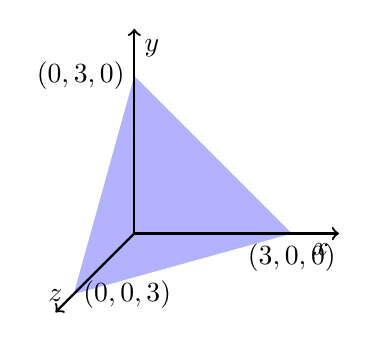
\begin{tikzpicture}
    \fill[blue, opacity=0.3] (2,0,0) -- (0,2,0) -- (0,0,2) -- cycle;
    
    \draw[thick,->] (0,0,0) -- (2.6,0,0) node[anchor=north east]{$x$};
    \draw[thick,->] (0,0,0) -- (0,2.6,0) node[anchor=north west]{$y$};
    \draw[thick,->] (0,0,0) -- (0,0,2.6) node[anchor=south]{$z$};
    
    \node at (2, 0, 0) [anchor=north] {$(3,0,0)$};
    \node at (0, 2, 0) [anchor=east] {$(0,3,0)$};
    \node at (0, 0, 2) [anchor=west] {$(0,0,3)$};
  \end{tikzpicture}  
\]
for the above example minimum is at $(3,0,0)$
\item \textbf{Interior Point Method$\rightarrow$Karmarkar}

it uses steepest descent idea and calculus to travel within the feasible set and choose optimum!

\item \textbf{Duality LP}

minization of $c^Tx$ over the constraints $Ax=b$ can also be solved as
\[\boxed{\min_{Ax=b,x>0} c^Tx }\longleftrightarrow  \boxed{ \max_{A^Ty\leq c}b^Ty}\]
both are equivalent hence known as dual problems
\begin{itemize}
    \item Weak Duality: $b^Ty \leq c^T x$, $\forall$ $x,y$ $\implies$ $\min(\max b^Ty)=\max(\min c^Tx)$
\end{itemize}
its known as minimax theorem or a saddle point at the optimum solution.

\item \textbf{Max Flow Problem/ Min Cut Problem}

Suppose we have following graph network and some fluid flows from source $S_i$ to sink $S_f$ edges represent the maximum fluid can pass through it find the max fluid that can reach from $S_i$ to $S_f$
\[
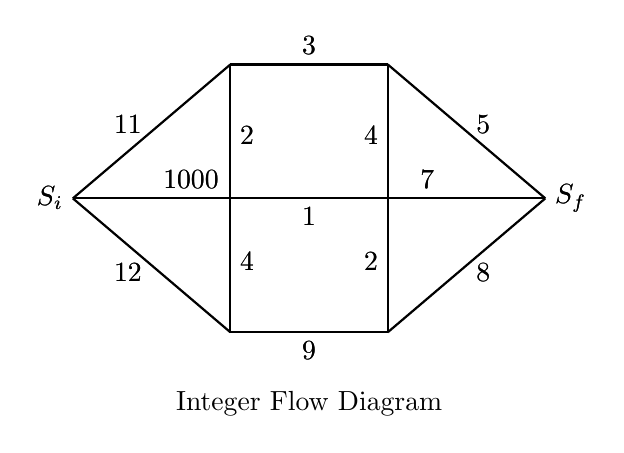
\begin{tikzpicture}

    \draw[thick,black] (-3,0) -- (3,0);
    \draw[thick,black] (-3,0) -- (-1,1.7);
    \draw[thick,black] (-1,1.7) -- (1,1.7);
    \draw[thick,black] (1,1.7) -- (3,0);

    \draw[thick,black] (-3,0) -- (-1,-1.7);
    \draw[thick,black] (-1,-1.7) -- (1,-1.7);
    \draw[thick,black] (1,-1.7) -- (3,0);

    \draw[thick,black] (-1,1.7) -- (-1,-1.7);
    \draw[thick,black] (1,1.7) -- (1,-1.7);


    \draw(-3,0) node[left]{$S_i$};
    \draw(3,0) node[right]{$S_f$};

    \draw(-2,0.7) node[above left ]{$11$};
    \draw(2,0.7) node[above right ]{$5$};
    \draw(-2,-0.7) node[below left ]{$12$};
    \draw(2,-0.7) node[below right ]{$8$};
    \draw(0,-1.7) node[below]{$9$};
    \draw(0,1.7) node[above ]{$3$};
    \draw(0,0) node[below]{$1$};
    \draw(-1.5,0) node[above]{$1000$};
    \draw(1.5,0) node[above]{$7$};

    \draw(-1,0.8) node[right]{$2$};
    \draw(1,0.8) node[left]{$4$};
    \draw(-1,-0.8) node[right]{$4$};
    \draw(1,-0.8) node[left]{$2$};
    \draw(-3,0) node[left]{$S_i$};
    \draw(3,0) node[right]{$S_f$};

    \draw(-2,0.7) node[above left ]{$11$};
    \draw(2,0.7) node[above right ]{$5$};
    \draw(-2,-0.7) node[below left ]{$12$};
    \draw(2,-0.7) node[below right ]{$8$};
    \draw(0,-1.7) node[below]{$9$};
    \draw(0,1.7) node[above ]{$3$};
    \draw(0,0) node[below]{$1$};
    \draw(-1.5,0) node[above]{$1000$};
    \draw(1.5,0) node[above]{$7$};

    \draw(-1,0.8) node[right]{$2$};
    \draw(1,0.8) node[left]{$4$};
    \draw(-1,-0.8) node[right]{$4$};
    \draw(1,-0.8) node[left]{$2$};

    \node at (0,-2.6) {{Integer Flow Diagram}};
\end{tikzpicture}
\]

\item \textbf{Two Person Game}

Suppose we have a following payoff matrix matrices for game I,II and III for persons $x,y$
\[
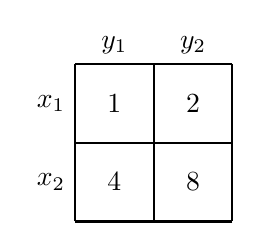
\begin{tikzpicture}
    % I
    \draw[thick,black] (-1,1) -- (1,1);
    \draw[thick,black] (1,1) -- (1,-1);
    \draw[thick,black] (1,-1) -- (-1,-1);
    \draw[thick,black] (-1,-1) -- (-1,1);

    \draw[thick,black] (-1,0) -- (1,0);
    \draw[thick,black] (0,1) -- (0,-1);

    \draw(0.5,0.5) node[]{$2$};
    \draw(-0.5,0.5) node[]{$1$};
    \draw(0.5,-0.5) node[]{$8$};
    \draw(-0.5,-0.5) node[]{$4$};

    \draw(-1,0.5) node[left]{$x_1$};
    \draw(-1,-0.5) node[left]{$x_2$};
    \draw(-0.5,1) node[above]{$y_1$};
    \draw(0.5,1) node[above]{$y_2$};

    % II

    % III
\end{tikzpicture}
\]
$x$ is going to play row wise while $y$ coloumn wise such that $x$ wants to minimize the sum of rows and $y$ wants to maximize the sum of columns

\textbf{Note:} it is zero sum game whatever one pays goes to other person only
\pagebreak
\begin{center}
    \textbf{\Huge{Lecture-20}}
\end{center}
\begin{center}
    \textbf{Prof. Suvrit Sra}
\end{center}
\item \textbf{Overview of Optimization Usecases}

Large scale machine learning deals with large no. of training data points and usually in higher dimensions mathematically we writes
\[\text{Training Data: } \{(x_1,y_1),(x_2,y_2)\dots,(x_n,y_n)\} \in \begin{bmatrix}
    \mathbb{R}^d \times n
\end{bmatrix}\]
in large scale machine learning $d,n$ are quite large.

Example-1: Least squares
\[\frac{1}{n}\left(\Vert Ax-b\Vert_2\right)^2=\frac{1}{n}\sum_{i=1}^{n}\left(a_i^Tx-b_i\right)^2=\frac{1}{n}\sum_{i=1}^{n}f_i(x)\]
Example-2: Lasso or $l_1$ least squares
\[\frac{1}{n}\left(\Vert Ax-b\Vert_2\right)^2+\lambda\Vert x\Vert_1=\frac{1}{n}\sum_{i=1}^{n}\left(a_i^Tx-b_i\right)^2+\lambda \sum_{j=1}^{d}\Vert x_j\Vert_1\]
Example-3: Support Vector Machine (SVM)
\[\frac{1}{2}(\Vert x\Vert)^2+\frac{C}{n}\sum_{i=1}^{n}max\left(0,1-y_i(x^Ta_i+b_i)\right)\]
all such examples can be written as \textbf{finite sum problems}

Example-4: Deep Neural Network(DNN)
\[\frac{1}{n}\sum_{i=1}^{n}loss\left(y_i,DNN(x:a)\right)=\frac{1}{n}\sum_{i=1}^{n}f_i(x)\]
Example-5: Maximum likelyhood estimation(MLE)
\[\frac{1}{n}\sum_{i=1}^{n}log-likelihood\left(x:a\right)=\frac{1}{n}\sum_{i=1}^{n}f_i(x)\]

\item \textbf{Stochastic Gradient Descent(SGD)}

we had gradient descent in which one iteration used to look likelyhood
\[x_{k+1}=x_k-s_k \nabla f(x_k)\]
and as a finite sum
\[x_{k+1}=x_k-s_k \frac{1}{n}\sum_{i=1}^{n} \nabla f_i(x)\]
but practically calculating gradient at each point takes hours even days to complete the algorithm.to overcome that we use SGD where we randomly pick an integer $i(k) \in$ $\{1,2\dots,n\}$ or in other words we just compute

\[\boxed{x_{k+1}=x_k-s_k \nabla f_{i(k)}(x_k)}\]

now each iteration become $n$ times faster!

\textbf{But:} why SGD works?

\textbf{Ans:} in begin SGD makes rapid progress but near the solution it varies alot or fluctuations are observed in the solution domain!

\textbf{Note:} in ML we don't only care about solution to optimisation problem but also care about how well it works on \textbf{unseen data}.

Example: Least Squares with $x\in \mathbb{R}$
\[\min_{}f(x)=\frac{1}{2}\sum_{i=1}^{n}\left(a_ix-b_i\right)^2\]
by solving $\nabla f(x)=0$ exact solution can be found as follows
\[x^*=\frac{\sum_{i=1}^{n}a_ib_i}{\sum_{i=1}^{n}(a_i)^2}\]

and minimum of $f_i(x)$ will be at $x_i=b_i/a_i$
\[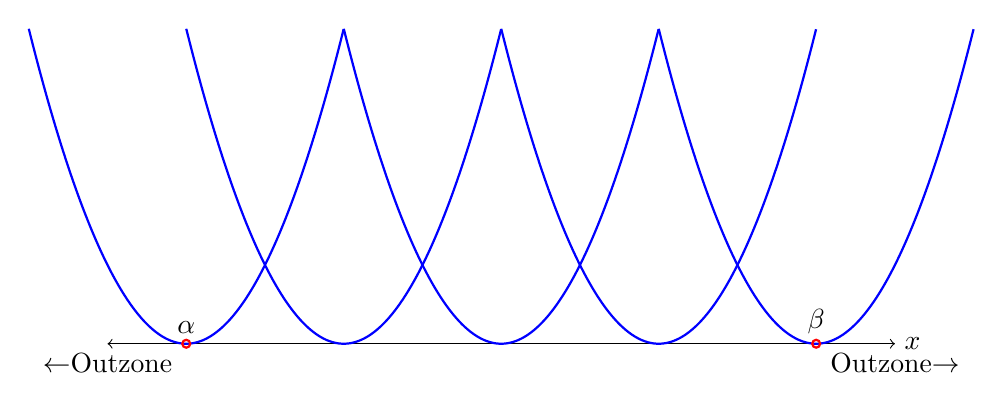
\begin{tikzpicture}
    \draw[<->] (-5,0) node[left]{}--(5,0) node[right]{$x$};
    \draw[
        domain=0:4,
        samples=100,
        smooth,
        variable=\x,
        blue,thick] plot({\x},{(\x-2)*(\x-2)});
    \draw[
        domain=-2:2,
        samples=100,
        smooth,
        variable=\x,
        blue,thick] plot({\x},{(\x)*(\x)});
    \draw[
        domain=-4:0,
        samples=100,
        smooth,
        variable=\x,
        blue,thick] plot({\x},{(\x+2)*(\x+2)});
    \draw[
        domain=-6:-2,
        samples=100,
        smooth,
        variable=\x,
        blue,thick] plot({\x},{(\x+4)*(\x+4)});
    \draw[
        domain=2:6,
        samples=100,
        smooth,
        variable=\x,
        blue,thick] plot({\x},{(\x-4)*(\x-4)});

        \draw(-4,0) node[above]{$\alpha$};
        \draw(4,0) node[above]{$\beta$};
        \draw(-5,0) node[below]{$\leftarrow$Outzone};
        \draw(5,0) node[below]{Outzone$\rightarrow$};
        \draw[thick,red] (4,0)circle[radius=0.05];
        \draw[thick,red] (-4,0)circle[radius=0.05];
\end{tikzpicture}\]

\textbf{Note$^1$:} that the solution minarg, $x^*$ $\in[\alpha,\beta]$, $\alpha=min(b_i/a_i),\beta=max(b_i/a_i)$ 

in the region $R=[\alpha,\beta]$ if we start the minization by picking a value of $x$ which is in far out region from $R$ then SGD will work kind of OK but as we enter $R$, SGD starts confusing 

\textbf{Note$^2$:} in 1-D if we are in far out region $\nabla f_i(x)$ has same sign as of $\nabla f(x)$ so using $\nabla f_i(x)$ instead of $\nabla f(x)$ we ensures our progress!

in higher dimensions the concept of sign changes to component $\nabla f_i(x)$ will have some component in the direction of true gradient $\nabla f(x)$.

\textbf{Note$^3$:} SGD uses \underline{stochastic} g\underline{radients} $g(x)$ such that the expection
\[\mathbb{E}(g(x))=\nabla f(x)\]

in expection $\mathbb{E}(g(x))$ is the true gradient instead of $\nabla f(x)$ also know as \textbf{unbiased estimate} of true gradient
\item \textbf{Varients of SGD}

\textbf{1.Point wise}
\begin{itemize}
    \item Pick an index $i \in \{1,2\dots,n\}$ without replacement OR
    \item Randomly pick an index $i \in \{1,2\dots,n\}$ with replacement
\end{itemize}
then use $g_k=f_i(x_k)$ as stochastic gradient for $x_{k+1}$

most of us uses version 2 which is no repetation of $i$ until we have gone through the entire training data set.\\
    
\textbf{2.Using mini Batches}
\[x_{k+1}=x_k- \frac{s_k}{\vert I_p \vert} \sum_{j \in I_p}^{}\nabla f_j(x_k)\]
where $\vert I_p \vert$ is size of mini batch we have choosen\\ 

\textbf{Note:} Very large mini batches not favorable for DNN.because then we'll end up over fitting the neural network and it won't be able to make pridictions for unseen data.

Here are few practical challenges which we often face while training the models using in this version of stochastic gradient descent
\begin{itemize}
    \item How to pich step size?
    \item Which mini batch to use?
    \item How to compute SGD? \textbf{Backpropogation}
    \item Gradient clipping!
    \item Adding momentum!
\end{itemize}

\begin{center}
    \textbf{\Huge{Lecture-21}}
\end{center}

\item \textbf{Neural Nets}

suppose we have an arbitrary vector $x\in \mathbb{R}^n$ and we want to create a function that seprates the space into two parts such that
\[f(x)=\begin{cases}
    <0 \hspace{5pt}, \text{1st Part}\\
    >0 \hspace{4pt}, \text{2nd Part}
\end{cases}\]

\textbf{Checkout Visual Examples$\longrightarrow$} \href{https://playground.tensorflow.org/#activation=tanh&batchSize=10&dataset=circle&regDataset=reg-plane&learningRate=0.03&regularizationRate=0&noise=0&networkShape=4,2&seed=0.67020&showTestData=false&discretize=false&percTrainData=50&x=true&y=true&xTimesY=false&xSquared=false&ySquared=false&cosX=false&sinX=false&cosY=false&sinY=false&collectStats=false&problem=classification&initZero=false&hideText=false}{Click Here}

Here are few basic Terminologies
\begin{itemize}
    \item Epoch: 1 iteration over the whole training data set
    \item Activation Function: Just a non linear function examples
    \begin{itemize}
        \item ReLu($r(x)$),sigmoid($\sigma(x)$),hyperbolic tangent ($t(x)$)
        \[r(x)=\max(0,x) \hspace{7pt}, \sigma(x)=\frac{1}{1+e^{-x}}\hspace{7pt}, t(x)=\text{tanh$x$}=\frac{e^x-e^{-x}}{e^x+e^{-x}}\]
    \end{itemize}
\end{itemize}
\pagebreak
Example of basic neural net with 1 layer

consider vector $x_0 \in \mathbb{R}^5$ is input element,and layer has 6 neurons then the output layer which here is just a single number this can be represented as 

\[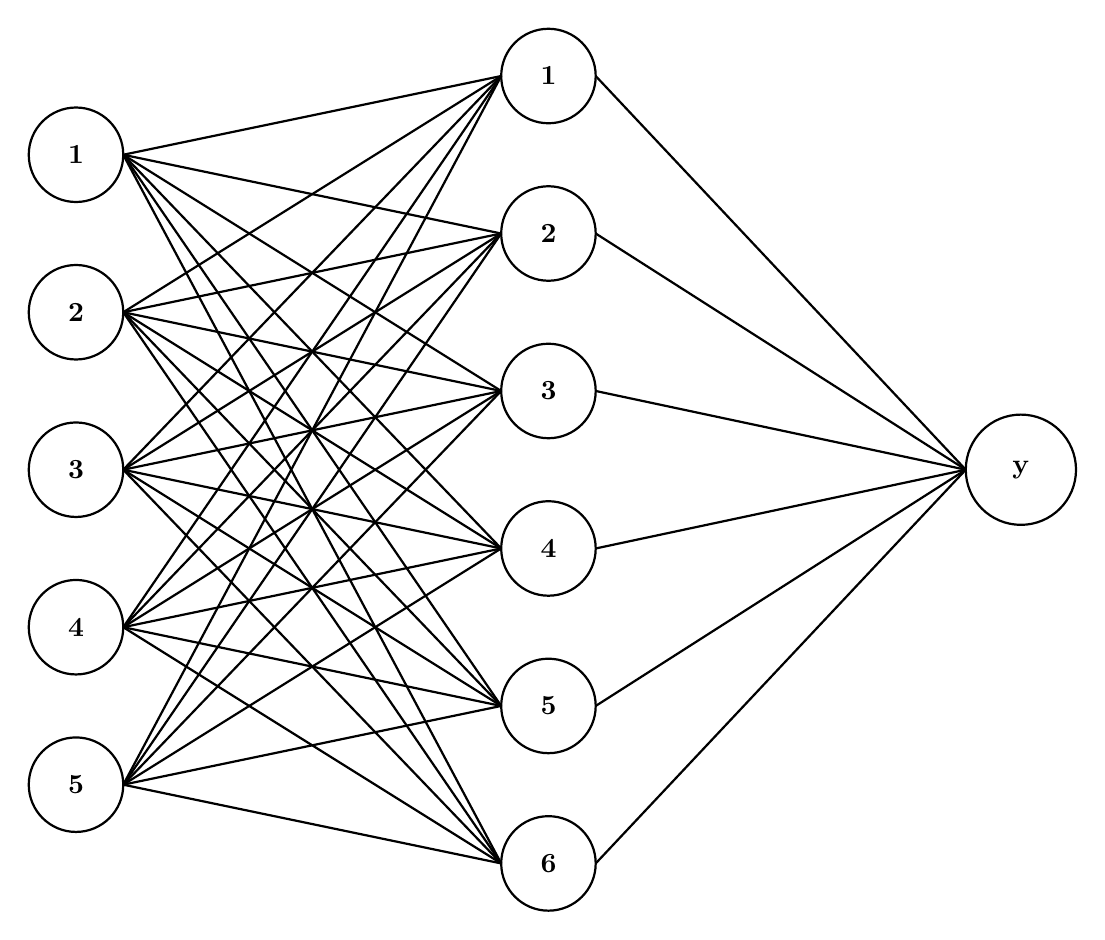
\begin{tikzpicture}
    \draw[thick,black] (-12,6)circle[radius=0.6];
    \draw[thick,black] (-12,4)circle[radius=0.6];
    \draw[thick,black] (-12,2)circle[radius=0.6];
    \draw[thick,black] (-12,0)circle[radius=0.6];
    \draw[thick,black] (-12,-2)circle[radius=0.6];


    \draw[thick,black] (-6,7)circle[radius=0.6];
    \draw[thick,black] (-6,5)circle[radius=0.6];
    \draw[thick,black] (-6,3)circle[radius=0.6];
    \draw[thick,black] (-6,1)circle[radius=0.6];
    \draw[thick,black] (-6,-1)circle[radius=0.6];
    \draw[thick,black] (-6,-3)circle[radius=0.6];

    
    \draw[thick,black] (0,2)circle[radius=0.7];

    \draw[thick,black] (-11.4,6) -- (-6.6,7);
    \draw[thick,black] (-11.4,6) -- (-6.6,5);
    \draw[thick,black] (-11.4,6) -- (-6.6,3);
    \draw[thick,black] (-11.4,6) -- (-6.6,1);
    \draw[thick,black] (-11.4,6) -- (-6.6,-1);
    \draw[thick,black] (-11.4,6) -- (-6.6,-3);

    \draw[thick,black] (-11.4,4) -- (-6.6,7);
    \draw[thick,black] (-11.4,4) -- (-6.6,5);
    \draw[thick,black] (-11.4,4) -- (-6.6,3);
    \draw[thick,black] (-11.4,4) -- (-6.6,1);
    \draw[thick,black] (-11.4,4) -- (-6.6,-1);
    \draw[thick,black] (-11.4,4) -- (-6.6,-3);

    \draw[thick,black] (-11.4,2) -- (-6.6,7);
    \draw[thick,black] (-11.4,2) -- (-6.6,5);
    \draw[thick,black] (-11.4,2) -- (-6.6,3);
    \draw[thick,black] (-11.4,2) -- (-6.6,1);
    \draw[thick,black] (-11.4,2) -- (-6.6,-1);
    \draw[thick,black] (-11.4,2) -- (-6.6,-3);

    \draw[thick,black] (-11.4,0) -- (-6.6,7);
    \draw[thick,black] (-11.4,0) -- (-6.6,5);
    \draw[thick,black] (-11.4,0) -- (-6.6,3);
    \draw[thick,black] (-11.4,0) -- (-6.6,1);
    \draw[thick,black] (-11.4,0) -- (-6.6,-1);
    \draw[thick,black] (-11.4,0) -- (-6.6,-3);

    \draw[thick,black] (-11.4,-2) -- (-6.6,7);
    \draw[thick,black] (-11.4,-2) -- (-6.6,5);
    \draw[thick,black] (-11.4,-2) -- (-6.6,3);
    \draw[thick,black] (-11.4,-2) -- (-6.6,1);
    \draw[thick,black] (-11.4,-2) -- (-6.6,-1);
    \draw[thick,black] (-11.4,-2) -- (-6.6,-3);

    \draw[thick,black] (-5.4,7) -- (-0.7,2);
    \draw[thick,black] (-5.4,5) -- (-0.7,2);
    \draw[thick,black] (-5.4,3) -- (-0.7,2);
    \draw[thick,black] (-5.4,1) -- (-0.7,2);
    \draw[thick,black] (-5.4,-1) -- (-0.7,2);
    \draw[thick,black] (-5.4,-3) -- (-0.7,2);
    
    \draw(-12,-2) node[]{\textbf{5}};
    \draw(-12,0) node[]{\textbf{4}};
    \draw(-12,2) node[]{\textbf{3}};
    \draw(-12,4) node[]{\textbf{2}};
    \draw(-12,6) node[]{\textbf{1}};

    \draw(-6,-3) node[]{\textbf{6}};
    \draw(-6,-1) node[]{\textbf{5}};
    \draw(-6,1) node[]{\textbf{4}};
    \draw(-6,3) node[]{\textbf{3}};
    \draw(-6,5) node[]{\textbf{2}};
    \draw(-6,7) node[]{\textbf{1}};

    \draw(0,2) node[]{\textbf{y}};
\end{tikzpicture}\]

\[y=A_2(A_1x_0+b_1)+b_2\]

where $y$ is output of order $1 \times 1$, $A_2$ is the matrix of order $1\times 6$ between layer 1 and output layer of, $A_1$ is a matrix of order $6 \times 5$ between input layer and layer 1, $x_0$ is input vector and $b_1,b_2$ are constant(called affines)\\

But in each neuron there are non linear activation function say ReLu for now which acts upon each entity they get

\begin{center}
    $y_1=A_1x_0+b_1$\\
    $\downarrow$\\
    $x_1=ReLu(y_1)$\\
    $\downarrow$\\
    $y_2=A_2x_1+b_2$\\
    $\downarrow$\\
    $y=x_2=ReLu(y_2)$
\end{center}

\textbf{Note:} For matrix $A_1$ have 30 free parameters and $A_2$ has 6 free parameters which we are trying to find by training the neural net\\
In general while training we have many layers between input and output.\\

More abstractly if we have $n$ layers then we have $n$-function composition where input vector $x\in \mathbb{R}^m$ 
\[f=f_n\left(f_{n-1} \dots \left(f_1(x)\right)\right) \hspace{3.5pt},\hspace{3.5pt} f_n(x)=ReLu\left(A_nx_{n-1}+b_n\right) \]

where each $f_i$ and $f$ is a \underline{continuous piecewise linear} function!\\

how many flat pieces we get if we are given or find $r(m,n)=?$
\begin{itemize}
    \item $r-$ no of flat pieces
    \item $m-$ dimensions of $x$
    \item $n-$ no of folds
\end{itemize}
\textbf{Example-1} if $m=1$ then $f(x)$ would look like where each critical point represents folds
\[\begin{tikzpicture}
    \draw[thick,black] (-3,0) -- (-1,-1);
    \draw[thick,black] (1,0) -- (-1,-1);
    \draw[thick,black] (1,0) -- (1.5,1.7);
    \draw[thick,black] (3,0) -- (1.5,1.7);
\end{tikzpicture}
r(1,n)=1+n
\]
\textbf{Example-2} if $m=2$ then $f(x)$ would look like where each region represent as plane and intersection lines represents folds
\[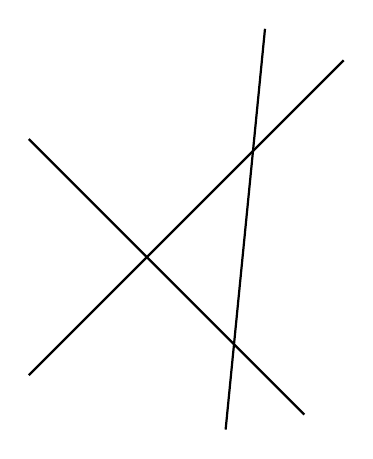
\begin{tikzpicture}
    \draw[thick,black] (-3,0) -- (1,4);
    \draw[thick,black] (0.5,-0.5) -- (-3,3);
    \draw[thick,black] (-0.5,-0.69) -- (0,4.4);
\end{tikzpicture} 
r(2,n)=1+\frac{n(n+1)}{2}
\]
\textbf{in General}
\[\boxed{r(m,n)=\binom{n}{0}+\binom{n}{1}\dots+\binom{n}{m}=\sum_{i=1}^{m} \binom{n}{i} \hspace{3.5pt}, m\leq n}\]

\textbf{Recurrence Relation}
\[\boxed{r(m,n)=r(m,n-1)+r(m-1,n-1)}\]
\pagebreak

\begin{center}
    \textbf{\Huge{Lecture-22}}
\end{center}
\item \textbf{Backpropogation}

it is just automatic differentiation reverse mode checkout \href{https://en.m.wikipedia.org/wiki/Automatic_differentiation}{Wikipedia!} and for more on reverse engineering checkout \href{https://colah.github.io}{Christopher-Olah Blogs!}

suppose we want to calculate partial differentiation of $f(x,y)$ w.r.t $x,y$ at $(2,3)$ where $f(x,y)$ is composition of $f_1,f_2,f_3$
\[f(x,y)=f_3(f_2(f_1(x,y)))=x^3(x+3y)\]
then 
\[\frac{\partial f}{\partial x}=\frac{\partial f_3}{\partial f_2}\frac{\partial f_2}{\partial f_1}\frac{\partial f_1}{\partial x}=4x^3+9yx^2 \hspace{4pt},\hspace{4pt} \frac{\partial f}{\partial y}=\frac{\partial f_3}{\partial f_2}\frac{\partial f_2}{\partial f_1}\frac{\partial f_1}{\partial y}=3x^3\]

Computational graph of $f(x)$
\[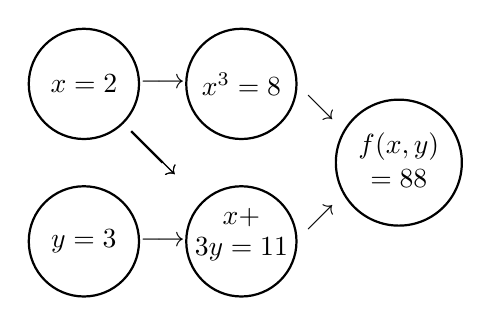
\begin{tikzpicture}
    \draw[thick,black] (-6,7)circle[radius=0.7];
    \draw[thick,black] (-6,5)circle[radius=0.7];
    \draw[thick,black] (-4,7)circle[radius=0.7];
    \draw[thick,black] (-4,5)circle[radius=0.7];
    \draw[thick,black] (-2,6)circle[radius=0.8];
    \draw(-5,7) node[]{$\longrightarrow$};
    \draw(-5,5) node[]{$\longrightarrow$};
    \draw(-5,6) node[]{${\searrow }$};
    \draw(-5,6) node[]{${\searrow }$};
    \draw(-3,6.7) node[]{$\searrow$};
    \draw(-3,5.3) node[]{$\nearrow$};
    \draw[thick,black] (-5.4,6.4) -- (-5,6);
    \draw(-6,7) node[]{$x=2$};
    \draw(-6,5) node[]{$y=3$};
    \draw(-4,7) node[]{$x^3=8$};
    \draw(-4,5.3) node[]{$x+$};
    \draw(-4,4.9) node[]{$3y=11$};
    \draw(-2,6.2) node[]{$f(x,y)$};
    \draw(-2,5.8) node[]{$=88$};
\end{tikzpicture}\]

similarly we can draw computational graph of partial derivative
and we found that reverse mode AD is much more efficient then forward mode\\
\[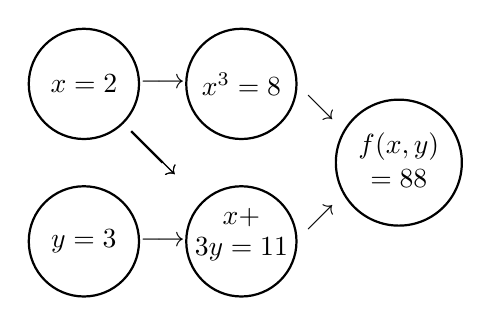
\begin{tikzpicture}
    \draw[thick,black] (-6,7)circle[radius=0.7];
    \draw[thick,black] (-6,5)circle[radius=0.7];
    \draw[thick,black] (-4,7)circle[radius=0.7];
    \draw[thick,black] (-4,5)circle[radius=0.7];
    \draw[thick,black] (-2,6)circle[radius=0.8];
    \draw(-5,7) node[]{$\longrightarrow$};
    \draw(-5,5) node[]{$\longrightarrow$};
    \draw(-5,6) node[]{${\searrow }$};
    \draw(-5,6) node[]{${\searrow }$};
    \draw(-3,6.7) node[]{$\searrow$};
    \draw(-3,5.3) node[]{$\nearrow$};
    \draw[thick,black] (-5.4,6.4) -- (-5,6);
    \draw(-6,7) node[]{$x=2$};
    \draw(-6,5) node[]{$y=3$};
    \draw(-4,7) node[]{$x^3=8$};
    \draw(-4,5.3) node[]{$x+$};
    \draw(-4,4.9) node[]{$3y=11$};
    \draw(-2,6.2) node[]{$f(x,y)$};
    \draw(-2,5.8) node[]{$=88$};
\end{tikzpicture}\]

\textbf{Note$^1$:} Another such fact can be observed in matrix multiplication means $A(BC)$ \text{can be efficient then} $(AB)C$ depending on the order of $A,B,C$

\textbf{Note$^2$:} No of operations required in $(A_{m\times n})\times (B_{n\times p})$ are $\boxed{mnp}$.
\pagebreak

\begin{center}
    \textbf{\Huge{Lecture-23}}
\end{center}

\item \textbf{Completing Rank 1 Matrix}

suppose we have to find all the entries of rank 1 matrix A of order $m\times n$ if we are given $m+n-1$ non zero entries of the martrix
\[A=uv^T\]
where $u\in \mathbb{R}^m$, $v\in \mathbb{R}^n$ and by choosing one of the entries of either $u$ or $v$ to be 1 we get $m+n-1$ are free variables in the matrix \\

\textbf{Note:} Whether we can find whole matrix or not depends on the position of each given element in $m+n-1$. take this example of $3\times 3$
\[A=\begin{bmatrix}
    x&x&x\\
    x&?&?\\
    x&?&?
\end{bmatrix} \hspace{4pt},\hspace{4pt} B=\begin{bmatrix}
    x &x&?\\
    x&x&?\\
    ?&?&x
\end{bmatrix}
\]

Note for matrix $A$ we can find $?$ setting determinant of sub matrix of $2\times 2$ to 0.but in case of $B$ we can't do it because determinant of matrix formed by $B_{11},B_{12},B_{21},B_{22}$ may or may not be 0.if it is zero which means we are given only 4 free variables instead of 5 if its not 0 that's not possible in since it is rank-1 matrix.\textit{But how to know by positions whether we'll be able to complete the matirx or not?} \\

\textbf{Bipartite Graphs}

if we make an undirected graph with source as row number and destination as coloumn number that will be a bipartite graph then if there is a cycle in graph then we can't complete the matrix! take example of $4\times 4$
\[A=\begin{bmatrix}
    x&x&x&x\\
    x&?&?&?\\
    x&?&?&?\\
    x&?&?&?
\end{bmatrix} \hspace{4pt},\hspace{4pt} B=\begin{bmatrix}
    x&?&?&x\\
    ?&x&?&x\\
    ?&?&x&?\\
    x&x&?&?
\end{bmatrix}\]
corrosponding bipartite graph of $A$ and $B$ would look like
\[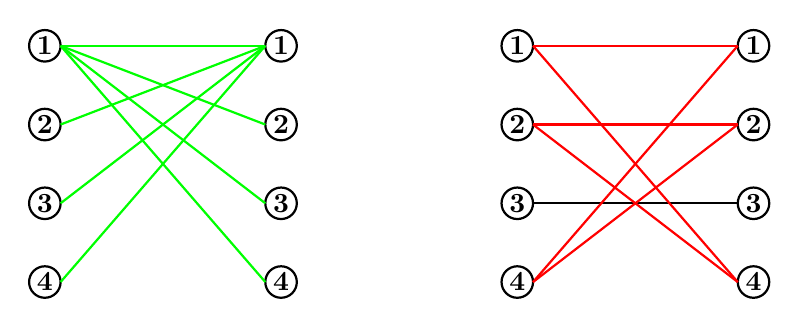
\begin{tikzpicture}
    \draw[thick,black] (-11,7)circle[radius=0.2];
    \draw[thick,black] (-11,6)circle[radius=0.2];
    \draw[thick,black] (-11,5)circle[radius=0.2];
    \draw[thick,black] (-11,4)circle[radius=0.2];


    \draw[thick,black] (-8,7)circle[radius=0.2];
    \draw[thick,black] (-8,6)circle[radius=0.2];
    \draw[thick,black] (-8,5)circle[radius=0.2];
    \draw[thick,black] (-8,4)circle[radius=0.2];

    \draw[thick,black] (-5,7)circle[radius=0.2];
    \draw[thick,black] (-5,6)circle[radius=0.2];
    \draw[thick,black] (-5,5)circle[radius=0.2];
    \draw[thick,black] (-5,4)circle[radius=0.2];


    \draw[thick,black] (-2,7)circle[radius=0.2];
    \draw[thick,black] (-2,6)circle[radius=0.2];
    \draw[thick,black] (-2,5)circle[radius=0.2];
    \draw[thick,black] (-2,4)circle[radius=0.2];

    \draw[thick,green] (-10.8,7) -- (-8.2,7);
    \draw[thick,green] (-10.8,7) -- (-8.2,6);
    \draw[thick,green] (-10.8,7) -- (-8.2,5);
    \draw[thick,green] (-10.8,7) -- (-8.2,4);

    \draw[thick,green] (-10.8,6) -- (-8.2,7);
    \draw[thick,green] (-10.8,5) -- (-8.2,7);
    \draw[thick,green] (-10.8,4) -- (-8.2,7);

    \draw(-11,7) node[]{\textbf{1}};
    \draw(-11,6) node[]{\textbf{2}};
    \draw(-11,5) node[]{\textbf{3}};
    \draw(-11,4) node[]{\textbf{4}};

    \draw(-8,7) node[]{\textbf{1}};
    \draw(-8,6) node[]{\textbf{2}};
    \draw(-8,5) node[]{\textbf{3}};
    \draw(-8,4) node[]{\textbf{4}};

    \draw(-5,7) node[]{\textbf{1}};
    \draw(-5,6) node[]{\textbf{2}};
    \draw(-5,5) node[]{\textbf{3}};
    \draw(-5,4) node[]{\textbf{4}};

    \draw(-2,7) node[]{\textbf{1}};
    \draw(-2,6) node[]{\textbf{2}};
    \draw(-2,5) node[]{\textbf{3}};
    \draw(-2,4) node[]{\textbf{4}};

    \draw[thick,black] (-4.8,5) -- (-2.2,5);

    \draw[thick,red] (-4.8,7) -- (-2.2,7);
    \draw[thick,red] (-4.8,6) -- (-2.2,6);
    \draw[thick,red] (-4.8,7) -- (-2.2,4);

    \draw[thick,red] (-4.8,6) -- (-2.2,4);
    \draw[thick,red] (-4.8,4) -- (-2.2,6);
    \draw[thick,red] (-4.8,4) -- (-2.2,7);
    
\end{tikzpicture}\]
in graph $A$ there is no cycle but in graph $B$ we does have a cycle
\pagebreak
\item \textbf{Circulant Matrix:Cyclic Convulution Matrix}

a general circulant matrix $C$ of order $n \times n$ looks like this
\[\begin{bmatrix}
    x_1&x_n&x_{n-1}&\dots&x_2\\
    x_2&x_1&x_{n}&\dots&x_3\\
    x_3&x_2&x_{1}&\dots&x_4\\
    \vdots&\vdots&\vdots&\ddots&\vdots\\
    x_n&x_{n-1}&x_{n-2}&\dots&x_1
\end{bmatrix}\]
\textbf{Note$^1$:} Every circulant matrix $C$ of order $n\times n$ can be written as sum of linear combinations powers of matrix $P$ of order $n\times n$, where $P$ shift one matrix of identity matrix is a permutation matrix as follows
\[P=\begin{bmatrix}
    0&1&0&0&\dots&0\\
    0&0&1&0&\dots&0\\
    0&0&0&1&\dots&0\\
    \vdots&\vdots&\vdots&&&\vdots\\
    0&0&0&0&\dots&1\\
    1&0&0&0&\dots&0\\
\end{bmatrix}\]
and $P_2$ is 2 shift matrix of identity and so on
\[C=c_0I+c_1P+c_2P^2\dots+c_{n-1}P^{n-1}=\left(\sum_{i=0}^{n-1}c_{i}P^{i}\right) \hspace{2pt},\hspace{2pt} P^0=I\]

\textbf{Note$^2$:} if $C,D$ are circulant matrices so the matrix $CD$ because $C,D$ are just polynomial of $P$ multiplication will also the polynomial of $P$.
\item \textbf{Convulution Operator}
\begin{itemize}
    \item \textbf{Non-Cyclic}: Take two vectors $(a,b,c)$ and $x,y,z$ then there non cyclic convulution is represented by operator ($\circledast$) and defined As
    \[(a,b,c)\circledast (x,y,z)=(ax,ay+bx,az+by+cx,bz+cy,cz)\]
    it can also be interpreted as multiplying two polynomial on LHS and writting the coefficients on RHS in vector form i.e.
    \[(a+bp+cp^2)(x+yp+zp^2)=\]
    \[(ax)+(ay+bx)p+(az+by+cx)p^2+(bz+cy)p^3+(cz)p^4\]

    \item \textbf{Cyclic}: it is define similar to non-cyclic except the fact that $p^n=1$ it is denoted by $\otimes$ taking the previous example
    \[(a,b,c)\otimes  (x,y,z)=(ax+byz+cy,ay+bx+cz,az+by+cx)\]
    it can also be interpreted as multiplying two polynomial on LHS and writting the coefficients on RHS in vector form i.e.
    \[(a+bp+cp^2)(x+yp+zp^2)=\]
    \[(ax)+(ay+bx)p+(az+by+cx)p^2+(bz+cy)p^3+(cz)p^4=\]
    \[(ax+by+cy)+(ay+bx+cz)p+(az+by+cx)p^2  \hspace{4pt}\because p^3=1,p^4=p\]
\end{itemize}
\pagebreak
\textbf{Note:} in cyclic and non cyclic both the convulution product of sum of elements of each argument is same as the sum of elements of output taking the previous example
\[(a+b+c)*(x+y+z)=ax+ay+bx+az+by+cx+bz+cy+cz\]
in general for any 2 vector $a,b$ convulution output $c$ has this property

    \begin{itemize}
    \item for Cyclic
\[\left(\sum_{i=0}^{n-1}a_i\right) \times \left(\sum_{i=0}^{n-1}b_i\right)=\sum_{i=0}^{n-1}c_i\]
    \item for Non-Cyclic
\[\left(\sum_{i=0}^{n-1}a_i\right) \times \left(\sum_{i=0}^{n-1}b_i\right)=\sum_{i=0}^{2n-2}c_i\]
    \end{itemize}

\item \textbf{Convulution of Continuos Functions}
\[\boxed{(f\ast g)(x)=f(x)\ast g(x)=\int_{-\infty}^{\infty}f(t)g(x-t)dt=\int_{-\infty}^{\infty}f(x-t)g(t)dt}\]

\item \textbf{Eigenvalues and Eigenvectors of Circulant Matirx}

Eigenvalues and eigenvectors of circulant matrix $C$ of order $n\times n$ are same a permutation matirx $P$such that
\[C=c_0I+c_1P+c_2P^2\dots+c_{n-1}P^{n-1}\]
but we know that eigenvalue of $P$ are $n^{th}$ roots of unity and eigenvectors matrix is same as fourier matrix($refer$ Page No.4 Reviewing Linear Algebra Section)

\textbf{Note:} Cyclicity of convulution in functions is seen by Periodicity!

\item \textbf{Toeplitz Matrix}

Matirx of type below are known as Toeplitz Matirx
\[T=\begin{bmatrix}
    t_0&t_1&\dots&\\
    t_{-1}&\ddots&\ddots&\vdots\\
    \vdots&\ddots&\ddots&t_1\\
    &\dots&t_{-1}&t_0
\end{bmatrix}\]
also know as Linear Shift Invarient(LSI) or Linear Time Invarient(LTI)!

in machine learning images have too many feature so that we use \textbf{max pooling}(in a small part we take max of that part for all bits)
\item \textbf{Matrix With Orthogonal Eigenvectors}
\begin{itemize}
    \item Symmetric Matrix: $A^T=A \rightarrow$ $\lambda=k+0i$
    \item Anti-Symmetric or Skew Symmetric Matrix: $A^T=-A \rightarrow$ $\lambda=0+ki$
    \item Orthogonal Matrix: $q_i^Tq_j=1$ only when $i=j$ else 0
    \item Diagonal Matrix: Matrix itself is eigenvector matrix.
    \item Normal Matrix: $A^TA=AA^T$
\end{itemize}
\pagebreak
\begin{center}
    \textbf{\Huge{Lecture-24}}
\end{center}
\item \textbf{Recap: Convulution Formula}
\[(c\ast d)_k=\sum_{i=0}^{n-1}c_id_{k-i} \hspace{3pt},\hspace{3pt}c \in \mathbb{R}^p,d\in \mathbb{R}^q\]
in non cyclic convulution there will be $p+q-1$ no. of terms in output and in case of cyclic convulution $p=q=n$ and no of term will be $n$
\item \textbf{2D Convulution of continuous functions}
\[(f\ast g)(x,y)=\int_{t}^{}\int_{u}^{}f(x,y)g(x-t,y-u)dudt\]
\item \textbf{Convulution Rule}

it shows the relation between point wise multiplication($.\ast$) and convulution($\circledast$) for fast fourier transform as follows
\[F(c\circledast d)=F(c).\ast F(d)\]
\boxed{\text{convolve then transform OR transform then multiply component wise}}\\

\textbf{Note$^1$:} \#Cost LHS=$n^2+nlogn$ and RHS=$2nlogn+n$\\
\textbf{Note$^2$:} Eigenvalues of $cd$ are same as product of eigenvalues of $c,d$
\item \textbf{Kronecker Product}

suppose we have two matrices $A,B$ order $n\times n$ each then 
\[K=Kron(A,B)=\begin{bmatrix}
    a_{11}B&a_{12}B&\dots&a_{1n}B\\
    a_{21}B&a_{22}B&\dots&a_{2n}B\\
    \vdots&\vdots&\ddots&\vdots\\
    a_{n1}B&a_{n2}B&\dots&a_{nn}B
\end{bmatrix}\]
\textbf{Note:} $K$ is a $n^2 \times n^2$ matrix \& $Kron(A,B)$ is Matlab Command

\item \textbf{Yet to complete the Lecture}
\begin{itemize}
    \item Kronecker Sum
    \item Laplacian
\end{itemize}
\pagebreak
\begin{center}
    \textbf{\Huge{Lecture-25}}
\end{center}
\item \textbf{Construction of Neural Nets:Learning Function}
\begin{itemize}
    \item Layer structure and features of input vector
    \[v_l=\psi  \left(A_{l}v_{l-1}+b_l\right))\]
    where $\psi$ is a non linear activation and $A_1,b_1,A_2,b_2\dots,A_l,b_l$ are unknowns, together represented as $x$ and in general number of unknowns(x) are greater than number of input features(v)\[\#x \gg \# v\]
    \item \textbf{Loss Function}
    \[L(x)=\frac{1}{n}\sum_{i=1}^{n}\left(F(x,v_i)-True_i\right)\]
    \item \textbf{Common Loss Functions}
    \begin{itemize}
        \item Square Loss: $L_2$ norm, used regression.
        \item Linear Loss: $L_1$ norms, used in lasso.
        \item Hinge Loss: used in $-1,1$ classification.
        \item Cross Entropy Loss: used in neural nets
    \end{itemize}
\end{itemize}
\item \textbf{Distance Matrices}

Question: Given the distance matrix($D$) of the points find the position matrix($X$) of points in $\mathbb{R}^d$. (note we have to find dimension, $d$ as well)
\[D_{ij}=\Vert x_i-x_j\Vert^2\]
Solution:
\[d_{ij}=\Vert x_i-x_j\Vert^2=(x_i,x_i)-(x_i,y_i)-(y_i,x_i)+(y_i,y_i)\]
\[\hspace{3cm} \uparrow \hspace{4cm} \uparrow\]
\[\hspace{2.7cm}  \text{Rank-1 Matrices depends only on $x$ or $y$}\]
so 
\[D=d\textbf{1}^T-2X^TX+\textbf{1}d^T\]

where \textbf{1} is column matrix of all 1's and now let matrix $G$ such that $G_{ij}$ represents dot product of $X_i,X_j$ or $G=X^TX$

\[X^TX=G=-\frac{1}{2}D+\frac{1}{2}d\textbf{1}^T+\frac{1}{2}\textbf{1}d^T\]

we can find X from G or $X^TX$ by following methods
\[X^TX=Q\varLambda Q^T \implies X=Q\sqrt{\varLambda}Q^T \tag*{Singular Value Decomposition}\]
\[X^TX=LDU=LDL^T \implies X=\sqrt{D}L^T \tag*{Cholesky Factorisation}\]

\textbf{Question:} Suppose $\Vert x_1-x_2\Vert^2=1$, $\Vert x_2-x_3\Vert^2=1$, $\Vert x_3-x_1\Vert^2=6$ clearly triangular inequlities are failing here go and figure out the issues!

\textbf{Solution:} 
\[D=\begin{bmatrix}
    0&1&1\\1&0&6\\1&6&0
\end{bmatrix}\]
let position matrix of $D$ is $X$ then it means that $X^TX=G$ is not positive semi-definate when triangular inequlities fails\\

\textbf{Note:} G is positive semi definate \boxed{\leftarrow iff\rightarrow} Triangular inequlities holds

\item \textbf{Procrustes Problem}

\textbf{Problem:} It is a problem of finding optimal rotation from one basis to other
suppose we have two set of basis vector in matrix form $X,Y$ find an orthogonal matrix $Q$ such that angular error is minimum
\[\min_{QQ^T=I} \left(\Vert YQ-X \Vert_F\right)^2\]
where $\Vert A\Vert_F$ is Frobenius norm of matrix $A$. Note we had following
\[\Vert A\Vert_F=\sum_{i=1}^{m}\sum_{j=1}^{n}(A_{ij})^2=\sum_{i=1}^{r} (\sigma_i)^2=trace(AA^T)=trace(A^TA)\]
\begin{itemize}
    \item $trace(AB)=trace(BA)$
    \item $trace(A^TB)=trace(B^TA)=trace(BA^T)$
\end{itemize}

\textbf{Solution:}
write SVD of $Y^TX$ as $u\Sigma v^T$ then $Q=uv^T$ proof yourself!

\item \textbf{Graph Clustring}

Finding a cut in graph that divides the graph into equal set of clusters!
for example to divide graph in 2 clusters $C_1,C_2$ we have to find $x,y$ s.t.
\[\left(\sum_{}^{}\Vert a_i-x\Vert^2+\sum_{}^{}\Vert b_i-y\Vert^2 \right) \text{ is minimum where, }a_i\in C_1,b_i\in C_2\]

\textbf{1. K-means Method:} Following steps are for 2-means
\begin{itemize}
    \item For given a's,b's find there centroids x,y.
    \item Given x's,y's form best clusters
    \item Repeat above steps
\end{itemize}
best cluster can be formed by using the fact that arbitrary point will go in the closer cluster.Check out the internet\\

\textbf{2. Spectral Clustering:} it starts by graph Laplacian matrix($L$)
\[L=A^TA=D-B\]
where $A$ is incidence matrix,$D$ is degree matrix,$B$ is adjacency matrix.
here are the definations of these matrices suppose we have following graph
\[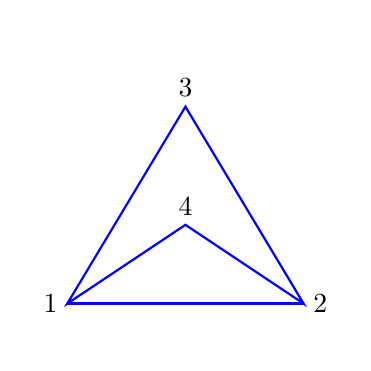
\begin{tikzpicture}
    \draw[very thin,gray] (-2,-2) (2,2);
    \draw[thick,blue] (1.5,-1.5) -- (0,1) --(-1.5,-1.5) --(0,-0.5)--cycle;
    \draw[thick,blue] (-1.5,-1.5) -- (1.5,-1.5);
    \draw(1.5,-1.5) node[right]{$2$};
    \draw(0,1) node[above]{$3$};
    \draw(-1.5,-1.5) node[left]{$1$};
    \draw(0,-0.5) node[above]{$4$};
\end{tikzpicture}
\]
\begin{itemize}
    \item \textbf{Incidence Matrix:} $-1$ represents source and 1 destination
    \[A=\begin{bmatrix}
        -1&1&0&0\\
        -1&0&1&0\\
        -1&0&0&1\\
        0&-1&1&0\\
        0&-1&0&1
    \end{bmatrix}\]
    \item \textbf{Degree Matrix:} It is a diagonal matrix with degree as entries
    \[D=\begin{bmatrix}
        3&0&0&0\\
        0&3&0&0\\
        0&0&2&0\\
        0&0&0&2\\
    \end{bmatrix}\]
    \item \textbf{Adjacency Matrix:} It denoteds the links between nodes
    \[B=\begin{bmatrix}
        0&1&1&1\\
        1&0&1&1\\
        1&1&0&0\\
        1&1&0&0
    \end{bmatrix}\]
    \item \textbf{Laplacian Matrix:} 
    \[L=D-B=\begin{bmatrix}
        3&-1&-1&-1\\
        -1&3&-1&-1\\
        -1&-1&2&0\\
        -1&-1&0&2\\
    \end{bmatrix}\]
\end{itemize}
Note matrix $L$ is not full rank and its nullspace is 1 dimensional and
\[Lx=0 \hspace{3pt}, x=\begin{bmatrix}
    c&c&\dots&c
\end{bmatrix}^T\]
so it has 1 eigenvalue as 0 and other are positive and eigenvector $y$ corrosponding to next eigenvalue greater than 0 is known as \textbf{Fiedler vector}

\textbf{Clustering:} Vector with positive components lies in one cluster and with negative components lies in other cluster

\textbf{Note:} $x,y$ are orthogonal because $L$ is symmetric P.S.D matrix
    \end{itemize}
\end{document}